% !TeX spellcheck = en_US
% !TeX root = ./0_article.tex

\documentclass[lettersize,journal]{IEEEtran}
\usepackage{amsmath,amsfonts}
\usepackage{algorithmic}
\usepackage{algorithm}
\usepackage{amsmath}
\usepackage{textgreek}
\DeclareFontFamily{U}{skulls}{}
\DeclareFontShape{U}{skulls}{m}{n}{ <-> skull }{}
\newcommand{\skull}{\text{\usefont{U}{skulls}{m}{n}\symbol{'101}}}
\usepackage{array}
\usepackage{mwe}
\usepackage{colortbl}
\usepackage{multirow}
\usepackage[caption=false,font=normalsize,labelfont=sf,textfont=sf]{subfig}
\usepackage{textcomp}
\usepackage{stfloats}
\usepackage{float}
\usepackage{url}
%\usepackage{natbib}
\usepackage{verbatim}
\usepackage{graphicx}
\usepackage{cite}
\usepackage{lipsum}
\usepackage{xcolor}
\usepackage{tabularx}
%\usepackage{subcaption}
%\usepackage{subfloat}
\usepackage{caption}
%\usepackage{subcaption}
\usepackage{fancybox}
\usepackage[utf8]{inputenc}

%\usepackage[inline]{showlabels}
\usepackage[final]{showlabels}

\hyphenation{op-tical net-works semi-conduc-tor IEEE-Xplore}
\def\BibTeX{{\rm B\kern-.05em{\sc i\kern-.025em b}\kern-.08em
		T\kern-.1667em\lower.7ex\hbox{E}\kern-.125emX}}
\usepackage{balance}

\begin{document}
%	\title{IEEE TCAD BBI ARTICLE (MAX 14 PAGES)}
	\title{Body biasing injection: analysis, modeling and simulation (MAX 14 PAGES)}
	\author{Geoffrey Chancel}
	\markboth{Journal of \LaTeX\ Class Files,~Vol.~3, No.~4, October~2077}%
	{Shell \MakeLowercase{\textit{et al.}}: A Sample Article Using IEEEtran.cls for IEEE Journals}
	\maketitle

	% !TeX spellcheck = en_US
% !TeX root = ./0_article.tex

\begin{abstract}
	This is the abstract.
\end{abstract}

\begin{IEEEkeywords}
	Article submission, IEEE, IEEEtran, journal, \LaTeX, paper, template, typesetting.
\end{IEEEkeywords}
	% !TeX spellcheck = en_US
% !TeX root = ./0_article.tex

\section{Introduction}
%\IEEEPARstart{S}{everal} researches have studied Body Biasing Injection (BBI) in the past few years.
%While this injection method had been \textcolor{orange}{paused/forgotten} for a few years, it has recently regained some interest.
%Among the latest studies, a modeling and simulation flow has been proposed, alongside better platforms allowing to achieve greater reproducibility and a deeper analysis of the mechanisms at works in digital integrated circuits subjected to BBI.
%In addition to that

%	\subsection{Context}
	\IEEEPARstart{N}{owadays}, electronic devices are found in every economic sector, and very often manipulate sensitive and confidential data, such as in bank transactions, Internet of Things (IoT) devices, smartcards, or smartphones.
	To ensure data authenticity and confidentiality, these devices embed cryptographic algorithms.
	While theoretically secure and robust, once implemented on actual devices, these algorithms become fallible by leaking the manipulated data through various physical quantities such as electromagnetic waves, infrared emissions, or sound emissions, not to cite them all, in addition to being sensitive to external disturbances.
	
	In this context, cybersecurity takes place, more specifically hardware security.
	When comes hardware security often comes side-channel attacks and fault injection attacks.
	On the one hand, side-channel attacks take advantage of the circuit leakage by measuring the various physical quantities available.
	On the other hand, fault injection aims at inducing physical disturbances into circuits, with methods like Electromagnetic Fault Injection (EMFI) \cite{mathieuEMFIFirst, mathieuEMFI}, Laser Fault Injection (LFI) \cite{lfiFaultModel}, or Body Biasing Injection (BBI) \cite{bbiOrigin}, not to cite them all.
	Among these methods, EMFI and LFI are widely studied and understood.
	However, despite a resurgence in the past few years, BBI knowledge is still less mature compared to the previously cited methods.
	Therefore, this article is dedicated in presenting our work on Body Biasing Injection.
	
%	\IEEEPARstart{W}{hen} working with cybersecurity, more specifically with hardware security, involving various integrated circuits ranging from smartcards, smartphones, or microcontrollers, various fault injection methods are often considered.
%	We can point out some of the most documented methods such as Electromagnetic Fault Injection (EMFI) \cite{mathieuEMFIFirst, mathieuEMFI}, Laser Fault Injection (LFI) \cite{lfiFaultModel}, or Body Biasing Injection (BBI) \cite{bbiOrigin}, not to cite them all.
%	Our work is dedicated in studying Body Biasing Injection.



	\subsection{Fault injection objectives}
		Before going further in the discussion about BBI, let us first outline the main objectives of fault injection methods.
		Most commonly, they are set up to perform various malicious manipulation on integrated circuits, such as:
		\begin{itemize}
			\item Denial of service (DoS) \textrightarrow\ Stop circuit operation and the related services;
			\item Verification bypass \textrightarrow\ Modify data on the fly to fake authenticity (e.g. to bypass bootloader security);
			\item Confidential data extraction \textrightarrow\ Modify data to perform differential fault analysis.
		\end{itemize}
		To perform these objectives, we can use various injection methods, such as EMFI, LFI or BBI.
		Before presenting our work on BBI further, let us analyze the available and existing BBI platforms in the state-of-the-art.
%		\textcolor{red}{To finish.}

	\subsection{BBI in the state-of-the-art}
	\textcolor{red}{Fait-on vraiment un paragraphe sur les plateformes industrielles comme dans la thèse ?}
		When compared to EMFI, BBI has a smaller state-of-the-art, whether in the amount of scientific papers published or in the amount of industrial platforms proposed.
		Currently, there are ten main works lingering on BBI \cite{bbiOrigin, bbiSecond, bbiThird, bbiColin,japbbi, japbbi2, mybbiCosade, mybbiFdtc2022, mybbifdtc2023, colinFdtc2023}.
		Each one of them made a unique contribution for a better understanding of BBI.

		The first one \cite{bbiOrigin} introduced the technique and presented a Bellcore attack on the targeted IC.
		Then, one year later, another work \cite{bbiSecond} further studied the method, followed by a third work three years later \cite{bbiThird}, introducing an advanced test bench to work and perform attacks with BBI.
		After that, another work presented a low-cost BBI platform, dedicated to WLCSP devices \cite{bbiColin}.

		However, there are still unanswered questions, and the current works aims at bringing more answers thanks to previous and new data.

		Before introducing the present work, let us eventually analyze the industrial platforms proposed by various manufacturers and introduce our own test platform.
		We can distinguish three major actors proposing BBI related products:
		\begin{itemize}
			\item Langer EMV-Technik;
			\item Riscure;
			\item NewAE Technology.
		\end{itemize}

		% !TeX spellcheck = en_US
% !TeX root = ./0_article.tex

\begin{figure}
	\centering
	\subfloat[][Langer]{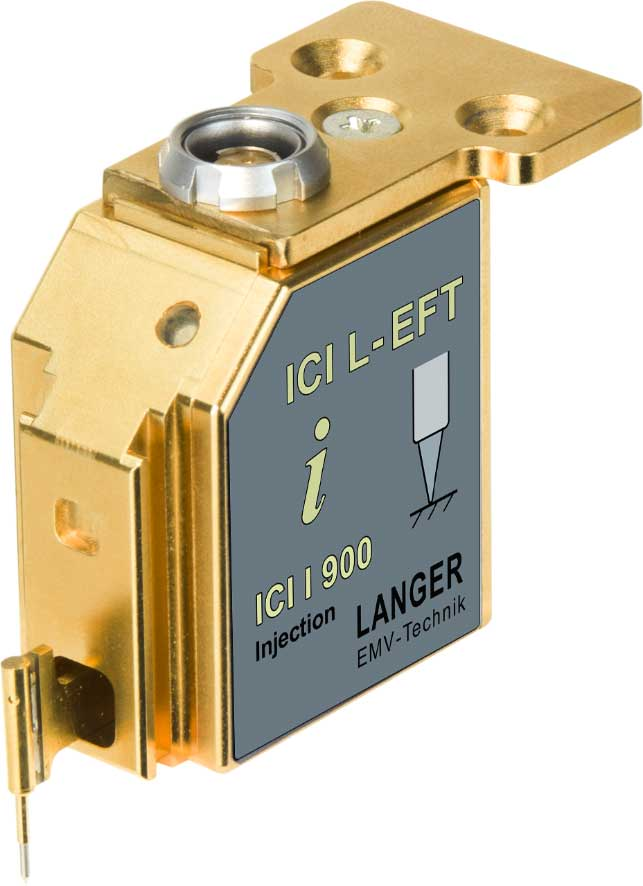
\includegraphics[width=0.2\columnwidth]{./figures/langerBBI.jpg}}
	\hspace{0.1\columnwidth}
	\subfloat[][Riscure]{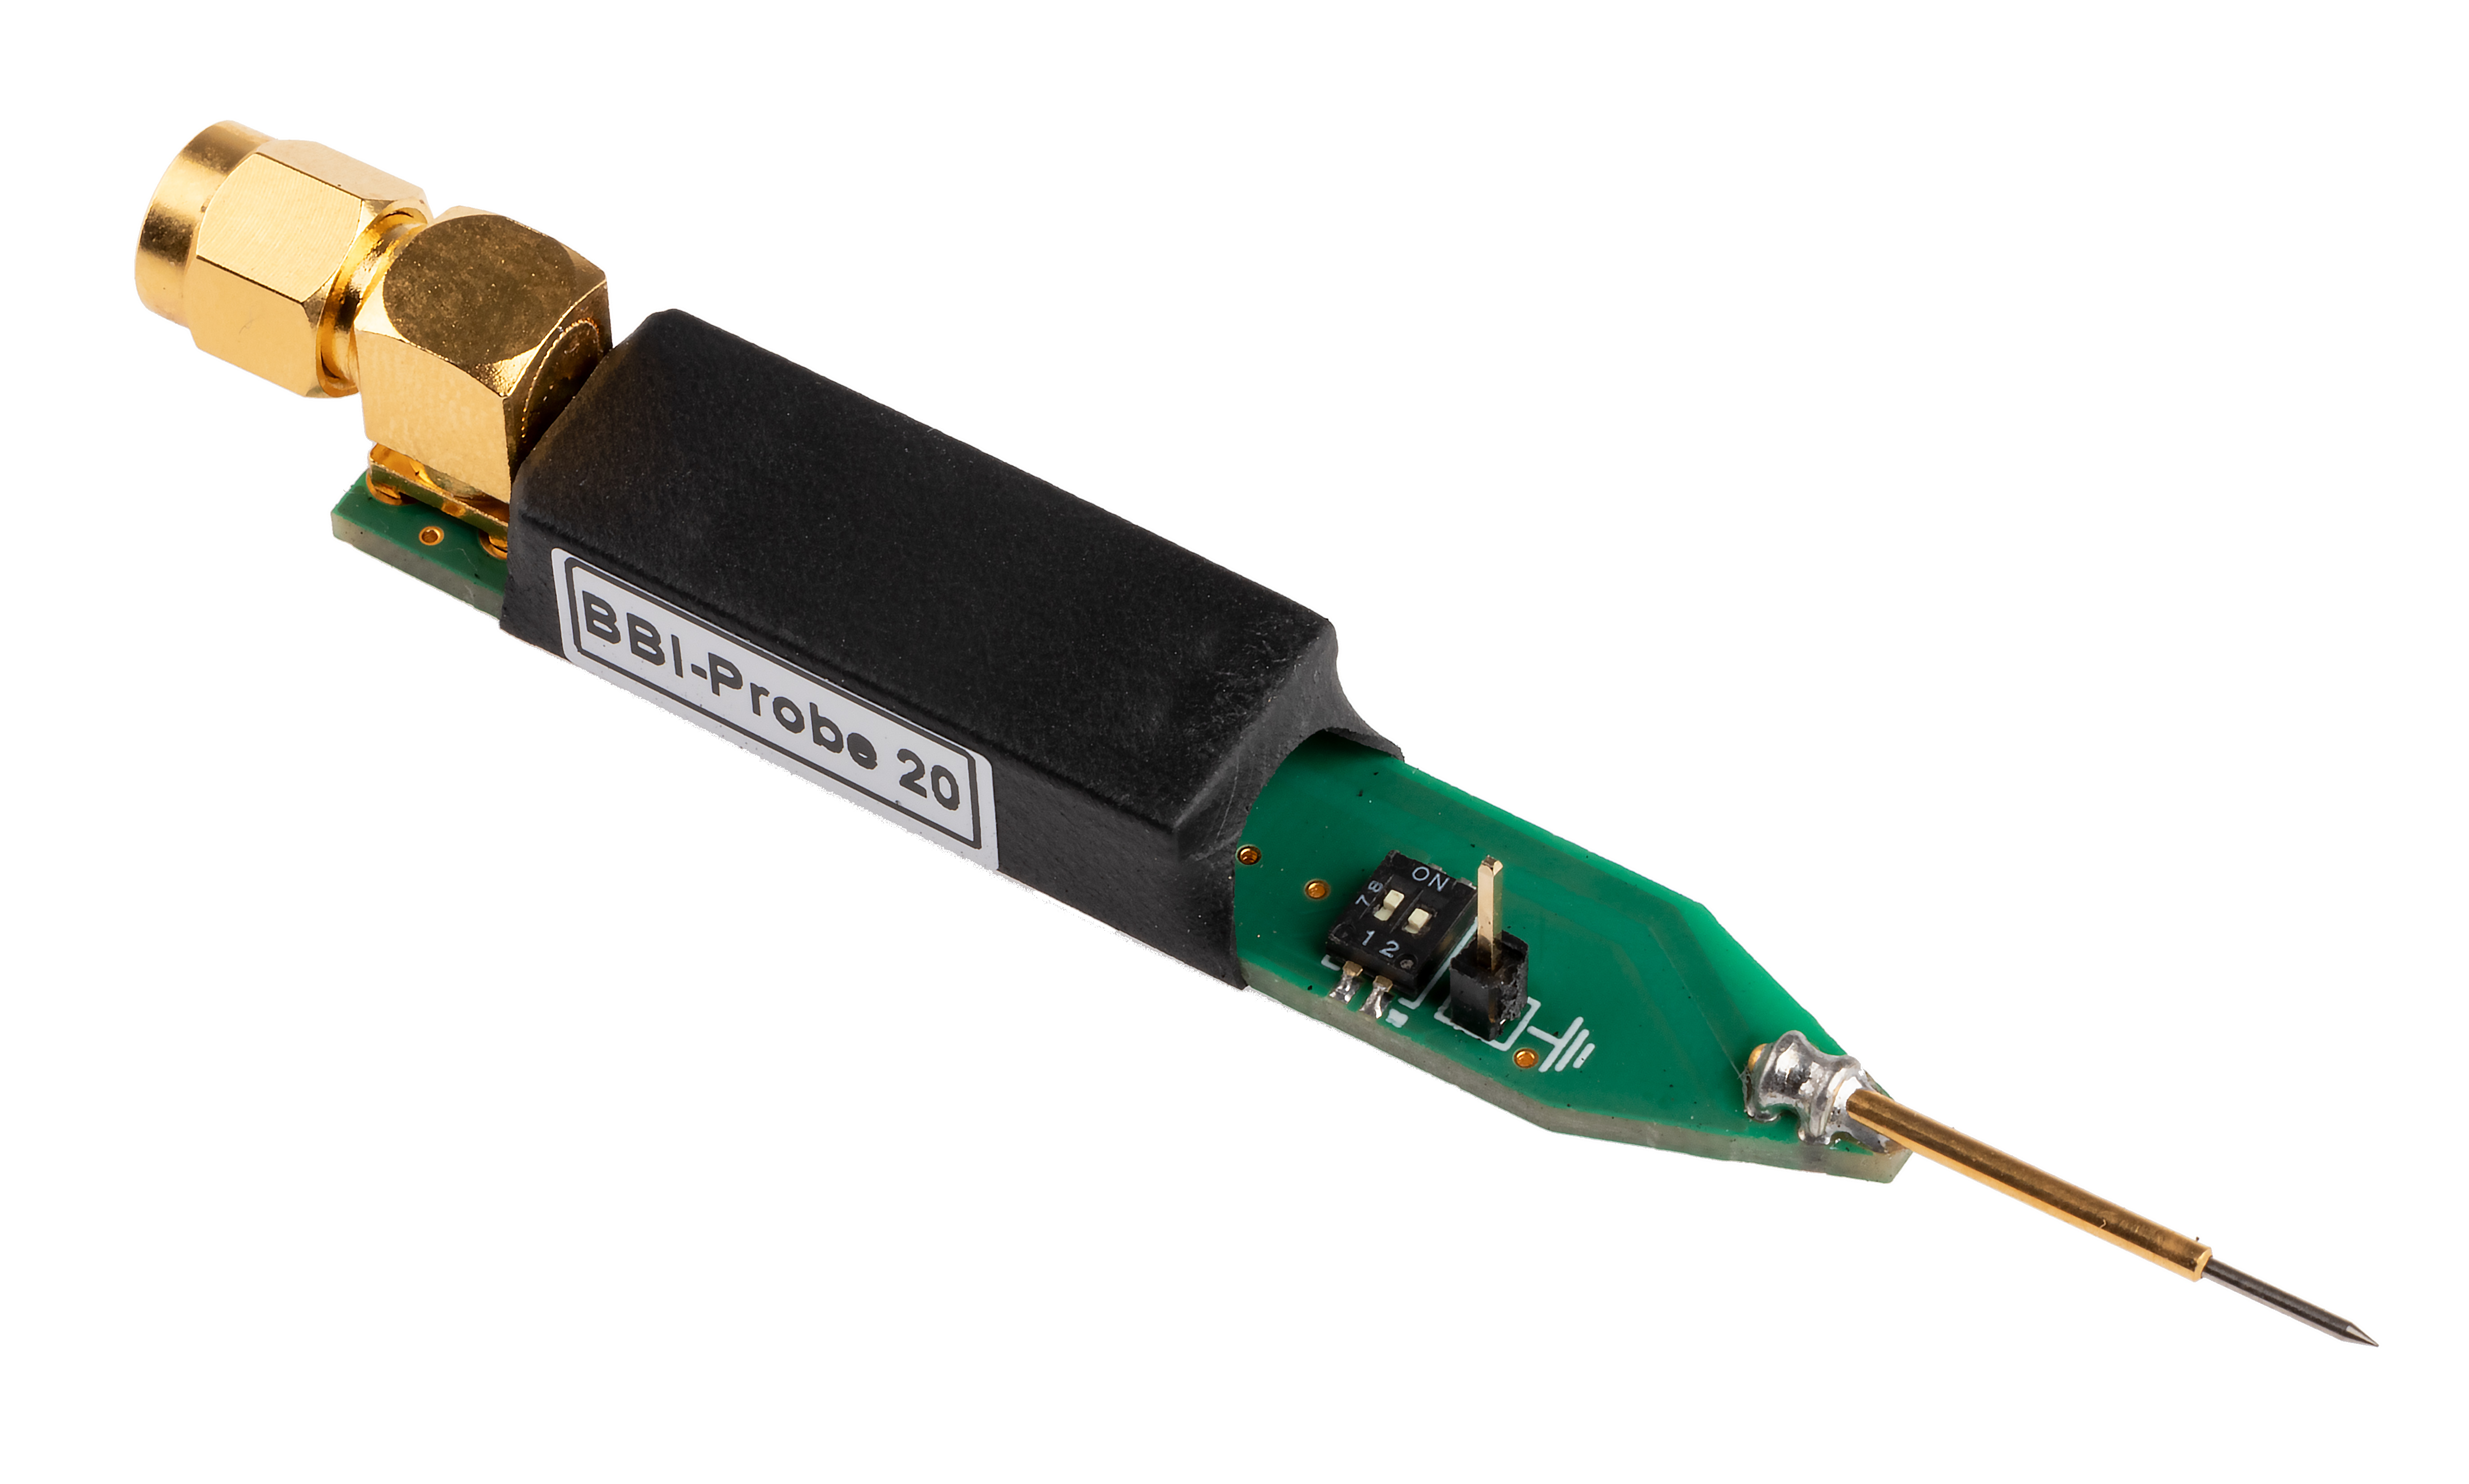
\includegraphics[width=0.425\columnwidth]{./figures/em-fi-bbi-probe-20-black.jpg}}
	\caption{Langer and Riscure BBI probes.}
	\label{riscure_langer}
\end{figure}
		\subsubsection{Langer EMV-Technik platform}
			The German society Langer EMV-Technik proposes an all-in-one and ready-to-use BBI platform composed of two hardware tools:
			\begin{itemize}
				\item A current pulse generator with a metal needle, shown in left in Fig. \ref{riscure_langer};
				\item A general controller called "Burst Power Station", combining a power supply, control and monitor tool and a software.
			\end{itemize}

	\subsection{BBI interrogations}
		With all the work in the state-of-the-art in mind, there are still remaining questions unanswered about BBI, such as:
		\begin{itemize}
			\item What is the spatial resolution of BBI?
			\item What is the time resolution of BBI?
			\item Is thinning the substrate useful in any way?
			\item How BBI induced faults occur?
			\item How to properly model BBI?
		\end{itemize}

	% !TeX spellcheck = en_US
% !TeX root = ./0_article.tex

\section{Practicing BBI in a better way}
	\IEEEPARstart{T}{his} section is dedicated in presenting BBI platforms and the various improvements which can be brought to a them to increase experiments repeatability and reliability.
	\subsection{BBI platforms in the state of the art}
		In the first place, we will analyze, from a theoretical perspective, a typical BBI platform, such as the one found in the state of the art.
		To do so, we created simple platform models highlighting the major limiting factors of such platforms.
		% !TeX spellcheck = en_US
% !TeX root = ./0_article.tex

\begin{figure}[h]
	\centering
	\subfloat[][Typical]{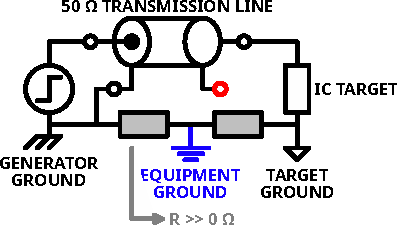
\includegraphics[width=0.5\columnwidth]{./figures/state-of-the-art-platform.pdf}}
	\subfloat[][Improved]{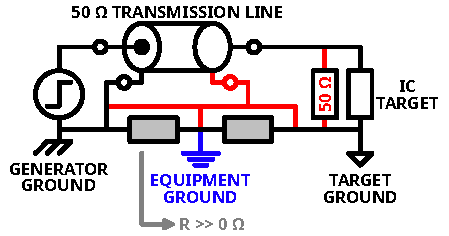
\includegraphics[width=0.5\columnwidth]{./figures/s-bbi-better.pdf}}
	\caption{Simple models of a typical (a) and an improved (b) BBI setup.}
	\label{bbi_setups}
\end{figure}

		The typical platform model is described in Fig. \ref{bbi_setups}a and shows the main components of a BBI platform, omitting positioning tables, such as:
		\begin{itemize}
			\item The voltage pulse generator;
			\item The transmission line;
			\item The grounding installation;
			\item The IC target.
		\end{itemize}
		In addition to this, the schematic in Fig. \ref{bbi_setups}a shows some important flaws we are going to address.

		While this is not always the case, fast and high-voltage pulse generators are typically specified to be loaded with a 50 \textOmega\ load, or more generally with a fixed load.
		When performing BBI, the backside of the IC is electrically connected to the generator output.
		Therefore, outside of luck alone, it is very rare that the impedance presented by the IC to the generator perfectly matches the required one.
		It implies that the generator will be, most of the time, out of specifications, and that the conditions will vary depending on the chosen IC, the substrate thickness, and the location of the BBI probe.
		This can lead to issues such as errors in the set-point voltage and pulse width, in addition to ringing in the transmission line.
		It then represents a first flaw to the typical approach.

		Then, there is the grounding installation.
		The model presents a non-ideal but simple platform grounding.
		The reference, used by the oscilloscope and the main computer, is represented in blue and called "equipment ground".
		Ideally, every ground on the platform is connected to this reference with a very low impedance interconnection.
		However, depending on the hardware used, it may greatly vary from one platform to another.
		In the model, the generator and target grounds are connected to the reference thanks to vastly imperfect interconnections, whose impedance is significantly greater than zero.
		This mainly lead to set-point errors due to shifts in the voltage pulse amplitude.
		Therefore, it limits the inter-platform repeatability and comparison of BBI experiments.

	\subsection{Our BBI platform}
		As most BBI platforms, our platform is focused on three main pieces of equipment: a voltage pulse generator, a metallic probe, and a positioning table.
		
		The positioning table we use is an OWIS PS 35 control unit, allowing to drive three motors for free movement in three dimensions.
		The generator model is the AVRK-4-B from the company Avtech Electrosystems Ltd.
		This model is commonly used for EMFI, but is suitable for BBI or any other application requiring fast voltage pulses, and its specifications are the following:
		\begin{itemize}
			\item Pulse amplitude: \textpm\ [150, 750] V;
			\item Pulse width: [6, 20] ns;
			\item First edge rise/fall time: 4 ns;
			\item Second edge rise/fall time: load dependent;
			\item Recovery time: \textless\ 1 ms;
			\item Propagation delay (PD): 150 ns;
			\item Jitter: \textpm\ 100 ps \textpm\ 0.03 \% of PD;
			\item DC-coupled output;
			\item Loaded with 50 \textOmega.
		\end{itemize}
		% !TeX spellcheck = en_US
% !TeX root = ./0_article.tex

\begin{figure}
	\centering
	\subfloat[][Global view]{\includegraphics[width=0.4\columnwidth]{./figures/sondeBBI_loin_raw.png}}
	\hspace{0.1\columnwidth}
	\subfloat[][Zoomed view]{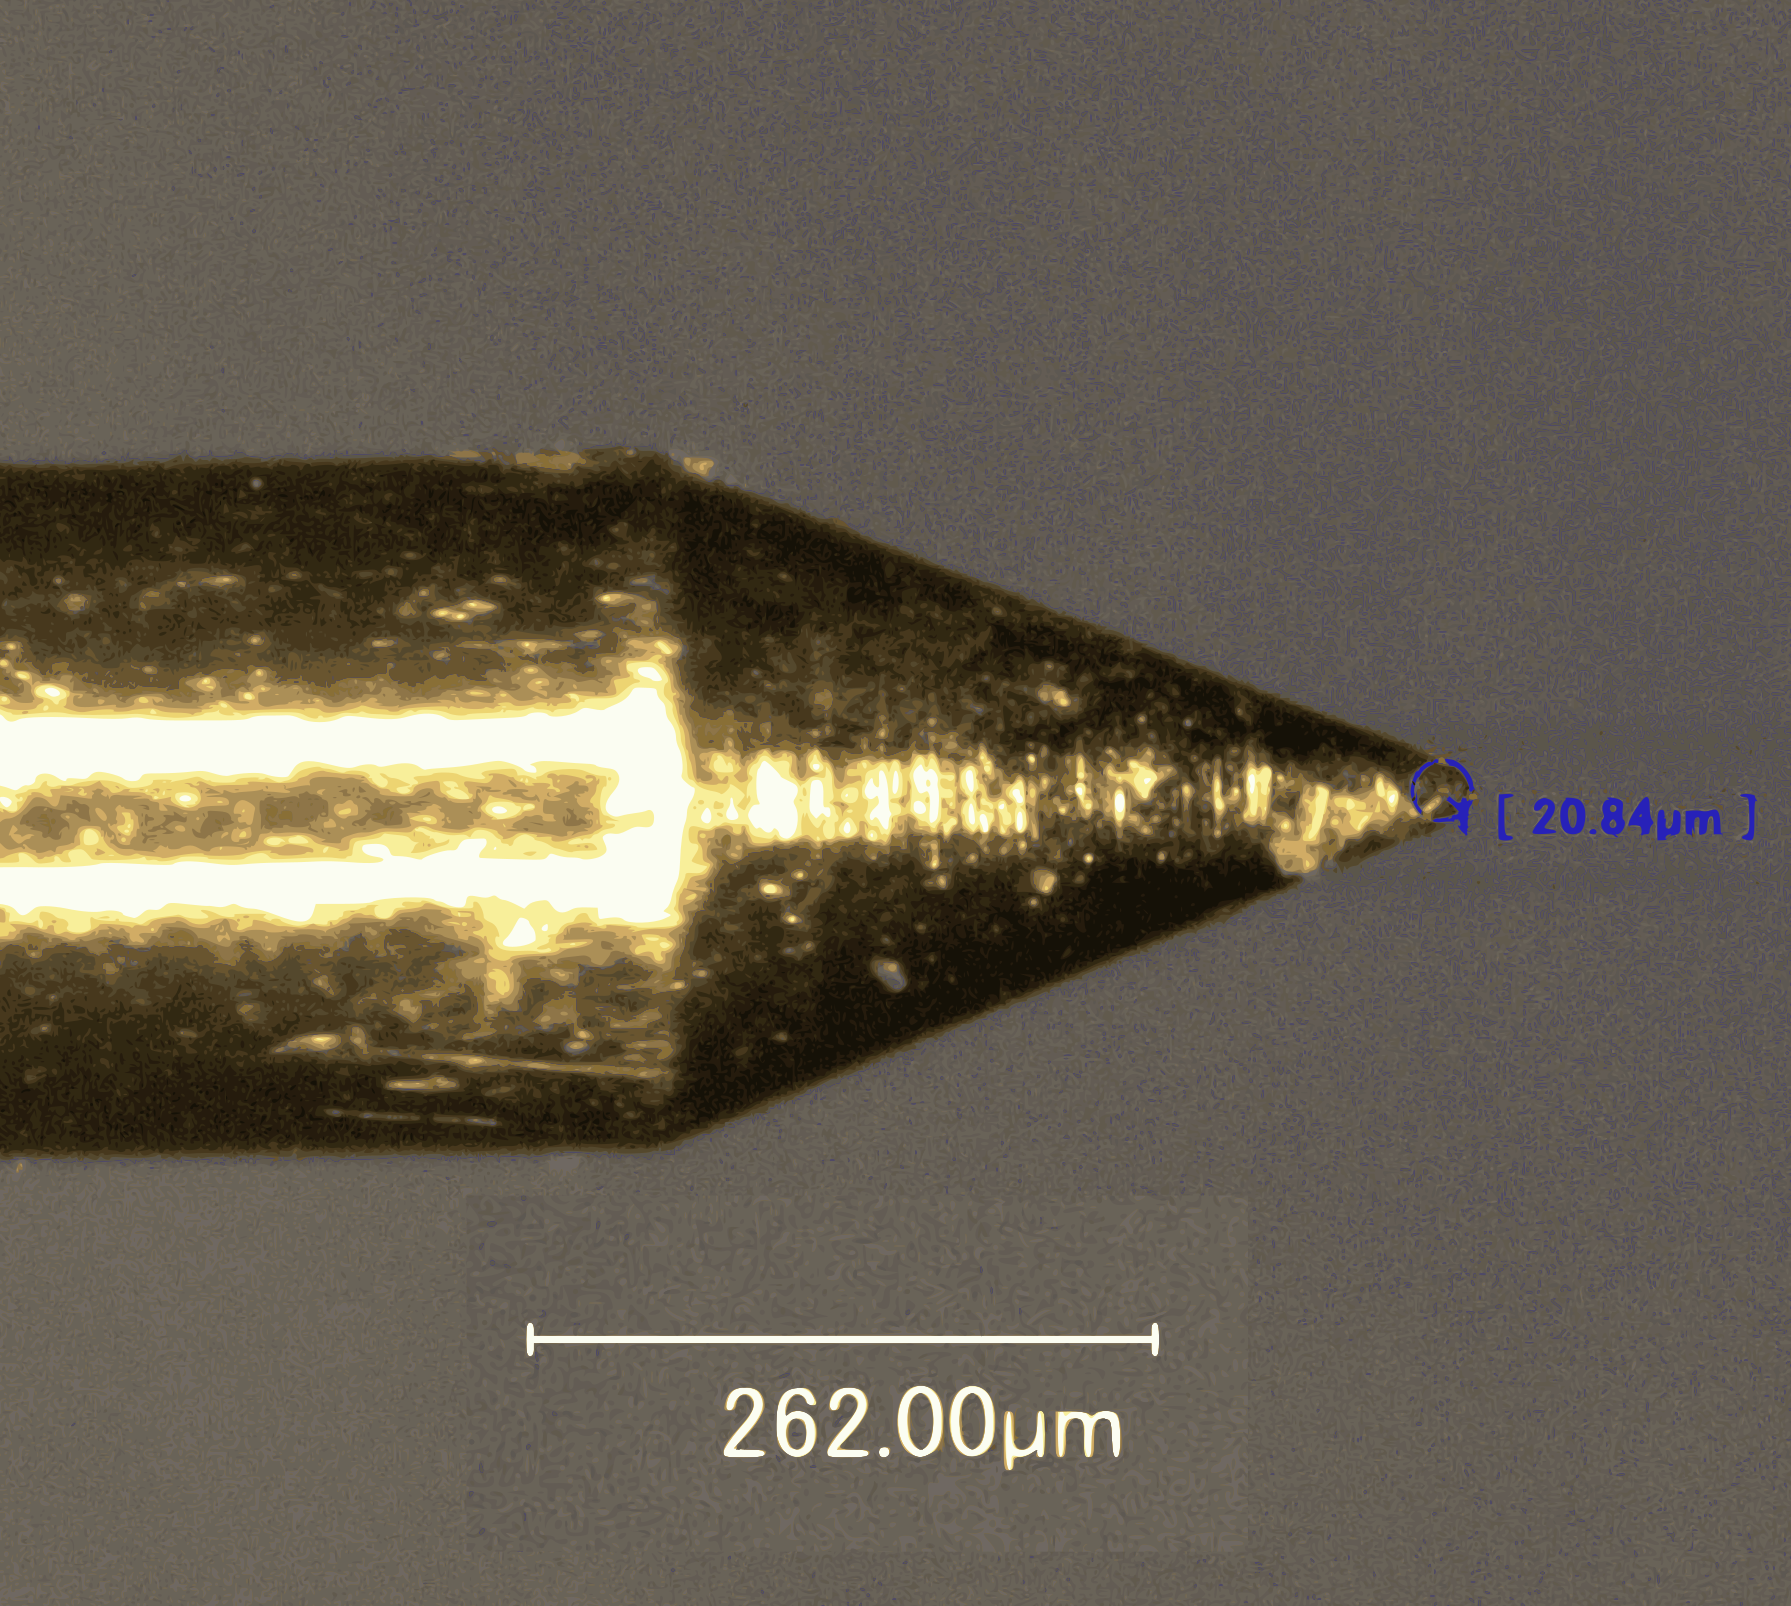
\includegraphics[width=0.4\columnwidth]{./figures/pointeBBI2.png}}
	\caption{Our custom BBI probe.}
	\label{bbi_probe}
\end{figure}
		Eventually, the most distinctive piece of equipment when it comes to BBI is the probe.
%		Probably the most distinctive piece of equipment when it comes top BBI is the probe.
		Some BBI probes can be active, others passive and less expensive.
		However, it is important to keep this piece of equipment relatively cheap as it endures most of the physical strain on a BBI platform, and should be easy to replace or repair.
		Fig. \ref{bbi_probe} shows two pictures of our probe from different angles.
		The one we use is custom-made around three parts:
		\begin{itemize}
			\item A spring-loaded metallic tip, with a 20 \textmu m head diameter;
			\item A SMA connector, where the tip is soldered;
			\item A custom 3D-printed enclosure holding the pieces together and cheap to replace.
		\end{itemize}
		The spring-loaded tip is 17 mm long and has a global diameter of 0.635 mm.
		It is specified for a 1.5 A nominal current, and its electrical resistance measures around 70 m\textOmega.
		The total cost of the probe is roughly of 20 \texteuro.

	\subsection{The proposed platform enhancements}
		To circumvent the previously introduced limitations, we propose two corrections to generalize the platforms and improve repeatability.

		First, let us talk about the generator impedance mismatch.
		For this purpose, multiple solutions can be approached.
		The best solution would be to implement an adaptive impedance matching system with active feedback, able to measure in real-time the impedance seen by the generator.
		However, adopting such a method is costly and long to set up in comparison to the next solution.
		Therefore, we propose a much simpler approach.
		Since, most of the time with our platform and targets, the impedance presented by the IC on its backside is in the order of 1 k \textOmega\ \cite{mybbifdtc2023}, approaching the 50 \textOmega\ expected by the generator can be done by connecting a 50 \textOmega\ resistor in parallel to the IC, as shown in the schematic in Fig. \ref{bbi_setups}b.
		
		Then, concerning the platform grounding, the solution is fairly straightforward.
		We propose to choose a reference, such as the equipment ground in our scenario, and bypass every other ground on the platform with low-impedance interconnections from the previously chosen reference, as proposed in Fig. \ref{bbi_setups}b.

%		First, let us talk about the improper grounding,
%		Alleviating this issue is fairly straightforward.
%		To do so, we propose to choose a reference, such as the equipment ground, and bypass all the grounds with low-impedance interconnections from this reference, as proposed in red in Fig. \ref{bbi_setups}.b.
%
%		Then, concerning the impedance mismatch of the generator, multiple solutions can be approached.
%		The best solution would be to implement an adaptive impedance matching system with active feedback, able to measure in real-time the impedance seen by the generator.
%		However, adopting such a method is costly and long to set up in comparison to the next solution.
%		Therefore, we propose a much simpler approach.
%		Since, most of the time, the impedance presented by the IC on its backside is in the order of 1 k\textOmega\, approaching the 50 \textOmega\ expected by the generator can be done by connecting in parallel to the IC a 50 \textOmega\ resistor, as it is shown in the schematic in Fig. \ref{bbi_setups}.b.

	\subsection{Platform enhancement validation}
		% !TeX spellcheck = en_US
% !TeX root = ./0_article.tex

\begin{figure}[h]
	\centering
%	\subfloat[][Typical]{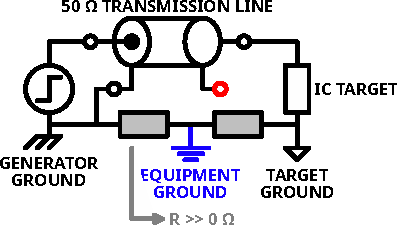
\includegraphics[width=0.5\columnwidth]{./figures/state-of-the-art-platform.pdf}}
%	\subfloat[][Improved]{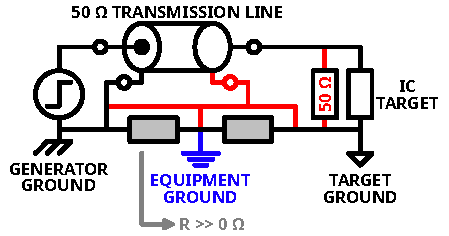
\includegraphics[width=0.5\columnwidth]{./figures/s-bbi-better.pdf}}
	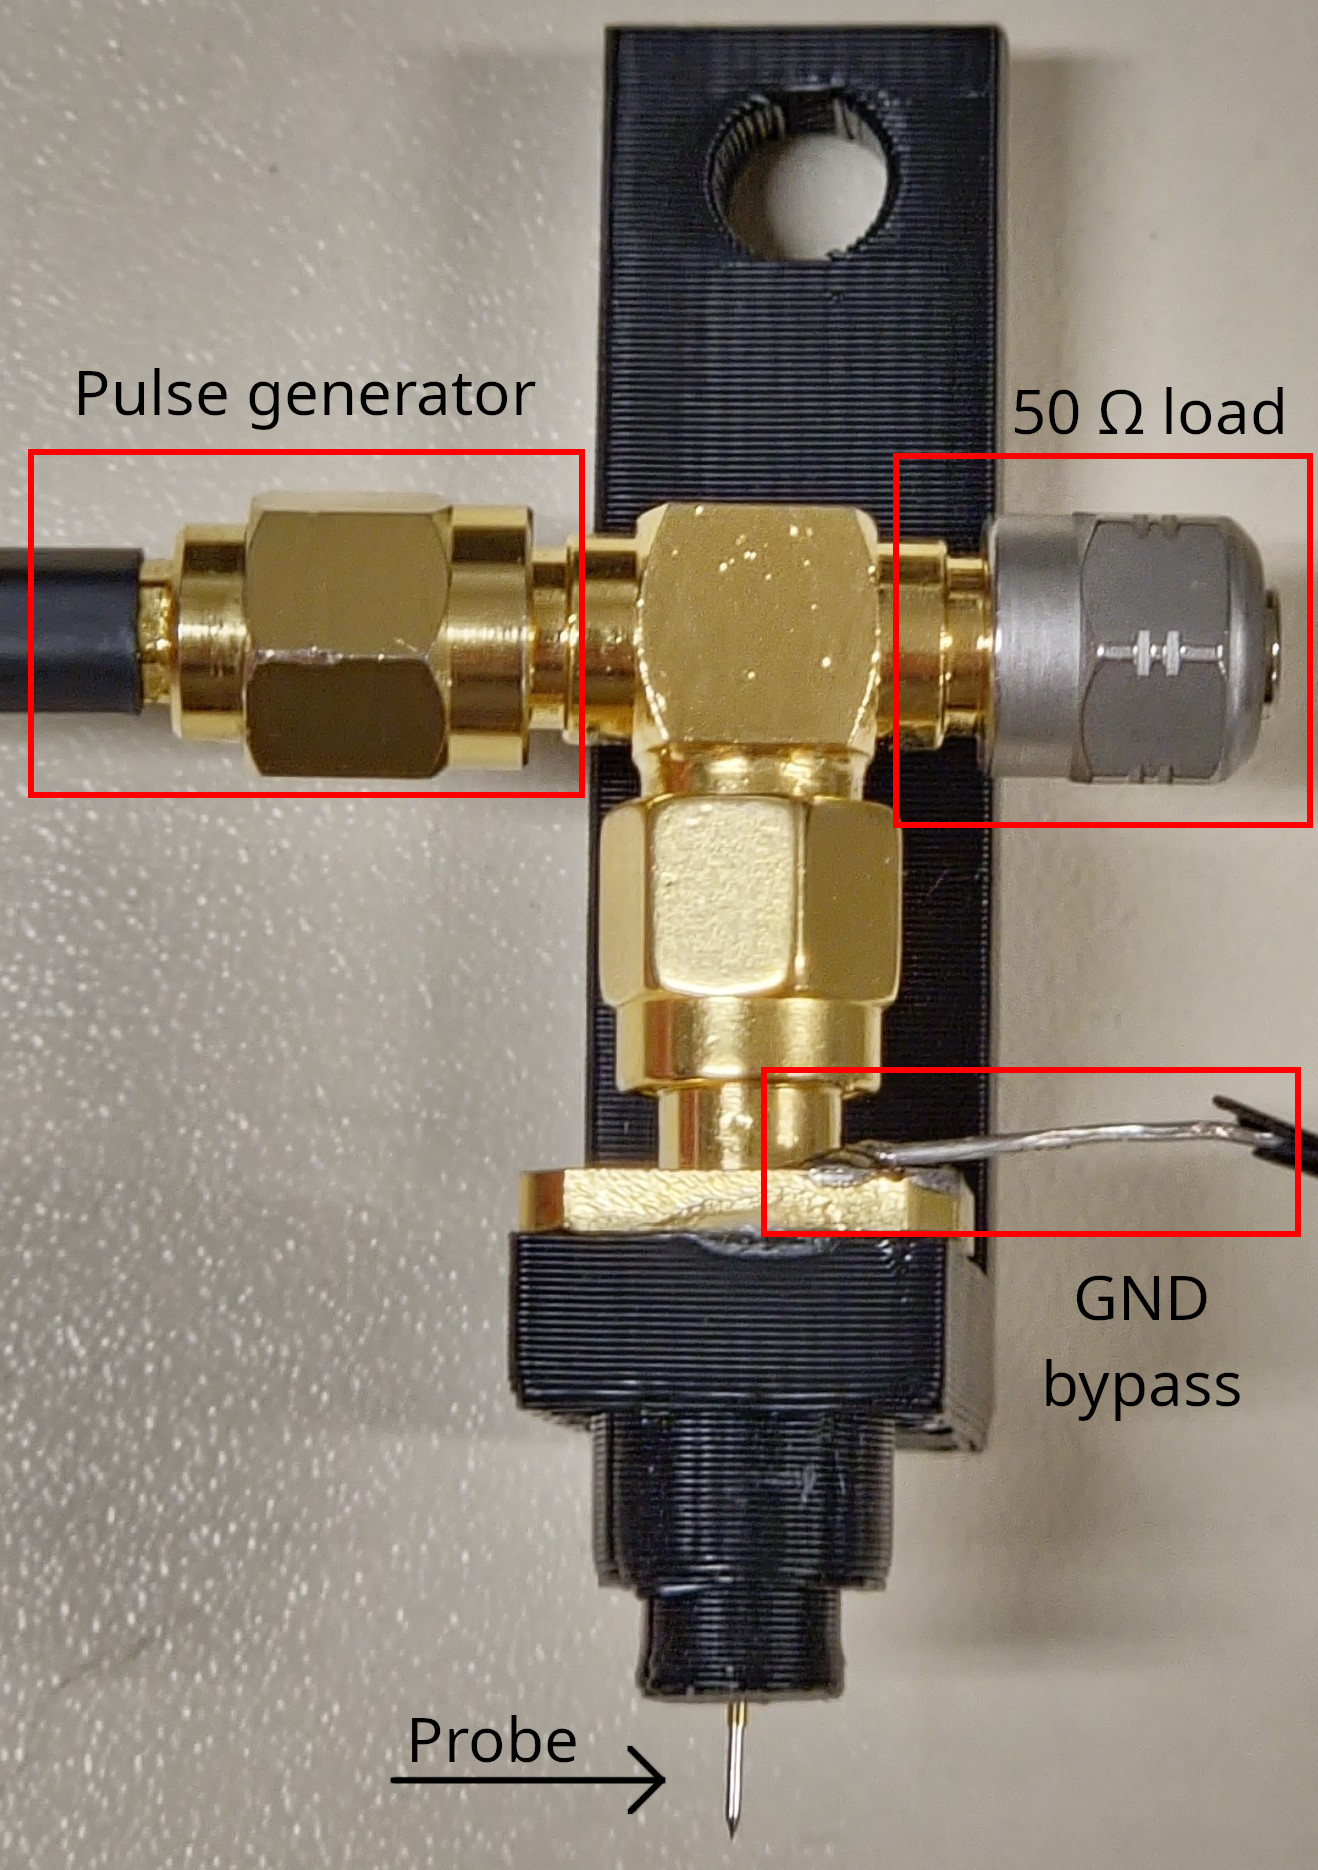
\includegraphics[width=0.40\columnwidth]{./figures/sondeGndSource.jpg}
	\caption{Impedance matching in practice.}
	\label{imp_match_real}
\end{figure}

		Now that we theoretically presented platform improvements, let us analyze their effective impact on our actual BBI platform.
		The proposed solution concerning the approximate impedance matching and ground bypassing is shown in Fig. \ref{imp_match_real}.
		The picture shows the BBI probe with a compensation load connected in parallel. in addition to the probe ground bypass.
		To show the actual interests of these improvements, let us analyze measured signals using our platform.

		We will compare before and after results and analyze the differences made by these improvements.
		To that end, we set up simple experiments consisting in injecting a voltage pulse into our IC target, measuring the voltage pulse at the probe and the current in the IC.
		% !TeX spellcheck = en_US
% !TeX root = ./0_article.tex

\begin{figure}[h]
	\centering
	%	\subfloat[][Typical]{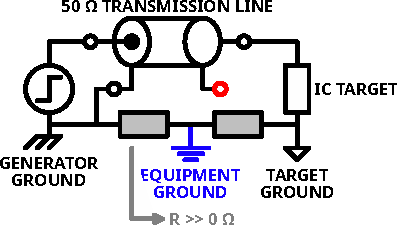
\includegraphics[width=0.5\columnwidth]{./figures/state-of-the-art-platform.pdf}}
	%	\subfloat[][Improved]{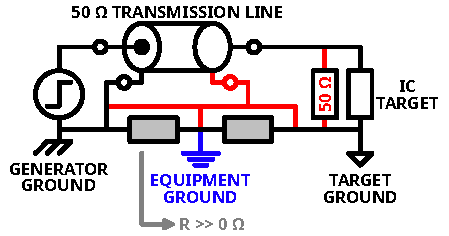
\includegraphics[width=0.5\columnwidth]{./figures/s-bbi-better.pdf}}
	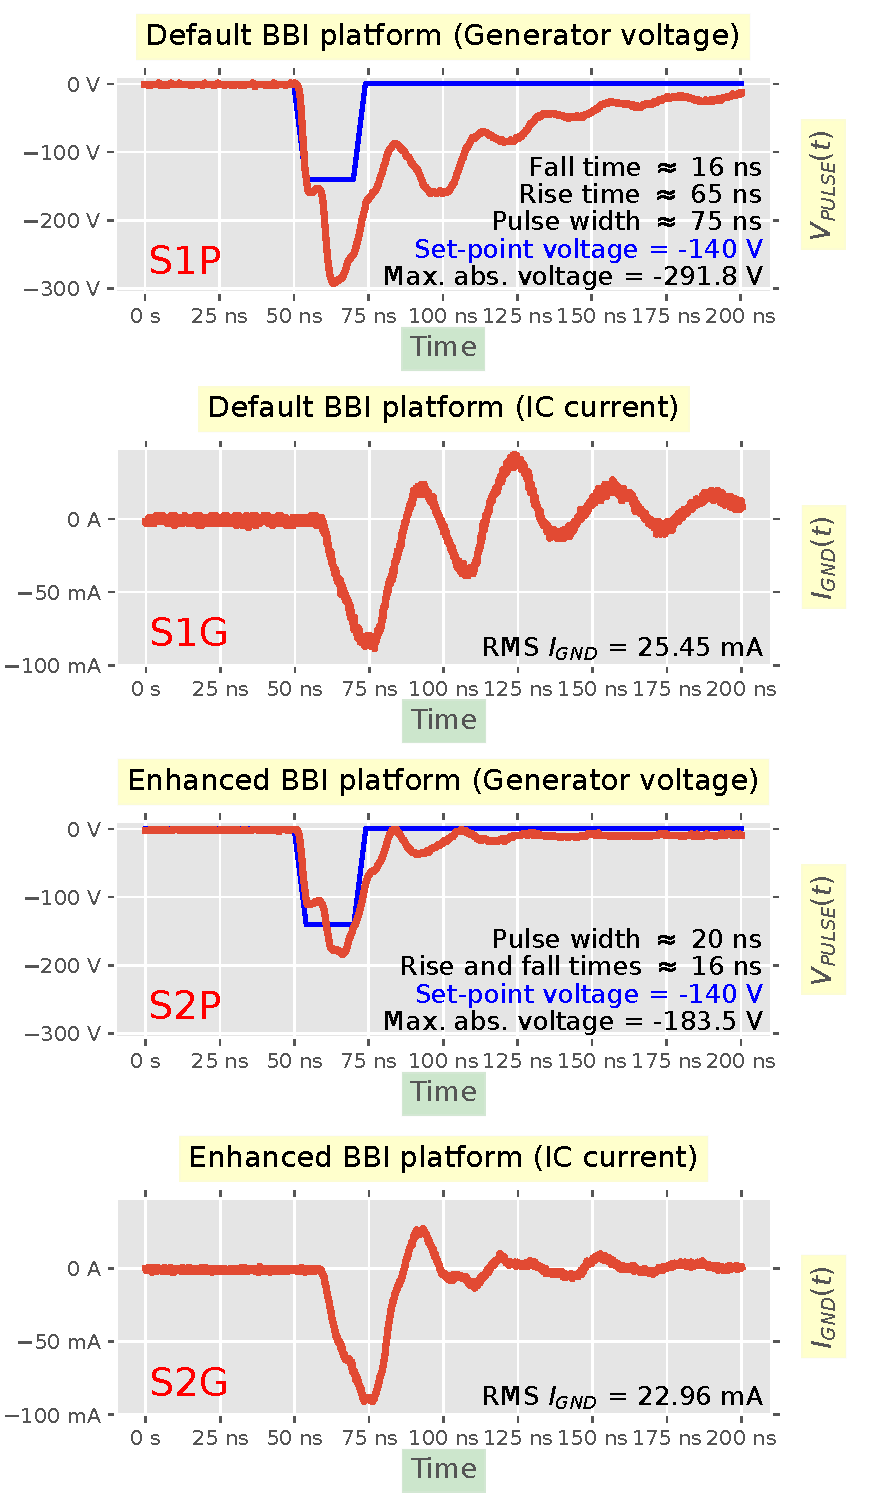
\includegraphics[width=\columnwidth]{./figures/realPulsesComparisons.pdf}
	\caption{Platform improvements in practice}
	\label{actual_imp}
\end{figure}

		Fig. \ref{actual_imp} presents the waveform results of such experiments.
		The figure shows four distinctive signals, in the following order:
		\begin{itemize}
			\item S1P: the voltage pulse before improvements;
			\item S1G: the IC ground current before improvements;
			\item S2P: the voltage pulse after improvements;
			\item S2G: the IC ground current after improvements.
		\end{itemize}
%		The figure is split in two main parts, the top row shows the results before the improvements, and the bottom row shows the results after the improvements.
		The experimental conditions are the following:
		\begin{itemize}
			\item Voltage pulse amplitude = -140 V;
			\item Voltage pulse width = 20 ns;
			\item Rise and fall times = 4 ns.
		\end{itemize}

		The waveform S1P shows in blue the ideal waveform according to the generator settings and in red the measured waveform.
		In addition to this are annotated some noteworthy values: such as the set-point voltage of -140 V, the max absolute measured voltage of 292 V, and rise and fall times.
		The first thing to notice here is the obvious undershoot of about -110 \% under the set-point.
		It is far from being desirable when performing fault injection as the voltage amplitude control is of great importance for precision purposes when considering the method effects on the IC \cite{mybbifdtc2023}.
		Furthermore, the pulse width is 275 \% higher than the set-point, measuring 75 ns instead of 20 ns.
		It is an additional issue as it annihilates the accuracy needed in this context, and leads to longer pulses injected into the IC, and therefore energy than required and uncontrollable behavior.
		Additionally, the rise and fall times are also 4 to 16 times higher than expected.
		Eventually, we can notice damped oscillations, an observation of ringing in the transmission line.

		Then, the waveform S1G, associated with the previous one, shows the IC ground current.
		Here, the damped oscillations are more clearly visible, in addition to the much longer than expected pulse duration.
		The RMS value of the injected current measures around 25 mA.

		Afterward, the waveform S2P shows the voltage results with the proposed improvements.
		The voltage pulse amplitude is much closer to the set-point, with an undershoot reduced to -31 \%.
		It is not perfect, but considering the simple nature of the impedance matching we propose, it was to be expected.
		On another note, the pulse width set-point is perfectly respected.
		However, the rise and fall times are still 4 times higher.
		
		Eventually, when looking at the S2G current waveform, we can remark the ringing reduction, while the amount of transferred energy remains approximately the same.

	\subsection{Platform enhancement application}
		To be able to illustrate further the actual interests of the proposed improvements, we did not only set up electrical measurements, but a complete differential fault attack (DFA).
		Indeed, performing fault injection is mainly used to perform attacks, therefore it makes sense to verify the soundness of the improvements in this context.
		We chose to perform a single bit DFA on our IC target, as the fault criterion is hard to obtain, and therefore it can easily show the interest, or the lack of interest, of performing such improvements to the platform.
		
		The target we used embeds a dedicated cryptographic core, which we set up using an AES on 128 bits.
		We then decided to perform the Giraud's DFA \cite{giraudDfa}, originally described in 2002.
		This attack requires creating single bit faults in one or more bytes on the targeted AES.
		Our target was clocked at 40 MHz thanks to an external 8 MHz crystal, and externally powered with 3.3 V.

		\subsubsection{Preliminary experiments}
			Before setting up the attack, we had to set up preliminary experiments allowing us to find optimal locations in the AES sub-circuit where the attack would be performed.
			Indeed, many areas and experimental parameters do not allow observing single-bit faults.
			
			To do so, we created what we call Fault Analysis Mappings (FAM).
			These experiments consist in creating maps of a specific region of the IC, in that case the AES sub-circuit, and analyzing the IC behavior while performing BBI for a set of various experimental parameters.
			We split the observed behavior into seven cases:
			\begin{itemize}
				\item Correct: the AES responds normally;
				\item Monobit Monobyte fault;
				\item Multibit Monobyte faults;
				\item Monobit Multibyte faults;
				\item Multibit Multibyte faults;
				\item Crash: the circuit did not respond correctly;
				\item Timeout: the circuit did not respond.
			\end{itemize}
			Therefore, as we only need single bit faults, only two cases are valid for the Giraud's DFA.
			To compare the two platforms, we performed a FAM on each one of them, using the following parameters:
			\begin{itemize}
				\item Pulse amplitude: from -150 V to -400 V with -5 V steps;
				\item Pulse width: 4.5 ns;
				\item Pulse delay: 150 ns + 553 ns targeting the penultimate AES round;
				\item Displacement step: 40 mm for the BBI probe over the mapped area.
			\end{itemize}
			Depending on the IC behavior, the experiments can take up to 36 hours.
			The parameters were chosen to minimize the maximum energy transferred into the IC to avoid damaging it as much as possible.
			% !TeX spellcheck = en_US
% !TeX root = ./0_article.tex

\begin{figure}[h]
	\centering
%		\subfloat[][Typical]{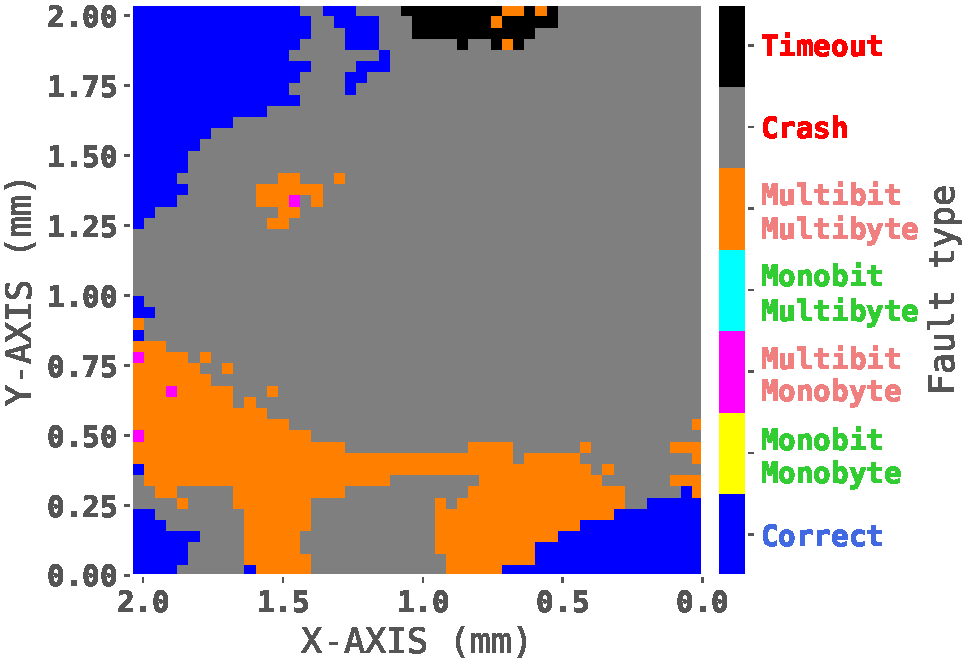
\includegraphics[width=0.5\columnwidth]{./figures/aesFastGndOnly-cropped.pdf}}
%		\subfloat[][Improved]{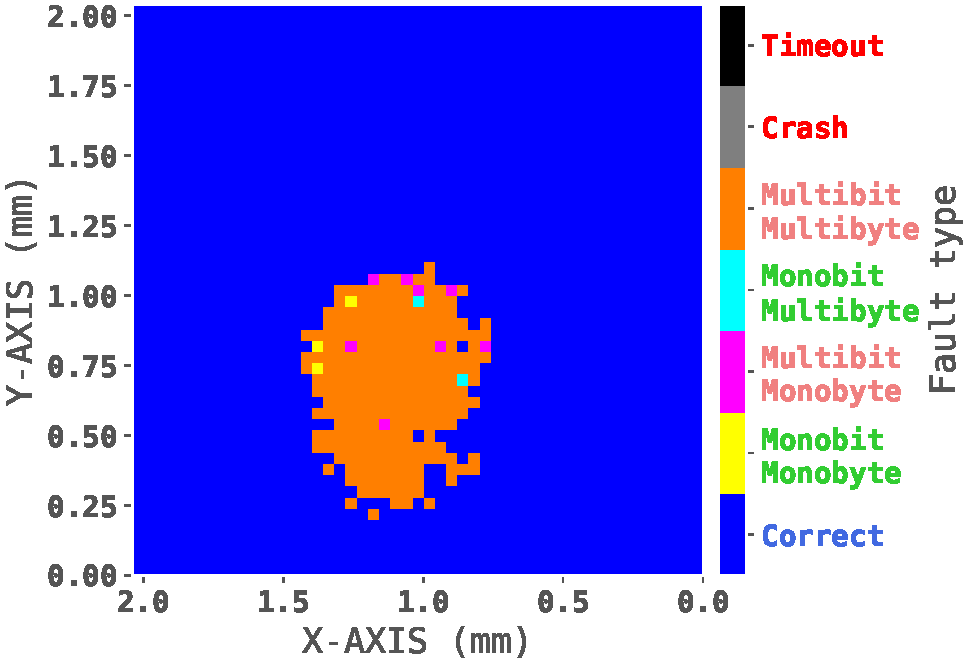
\includegraphics[width=0.5\columnwidth]{./figures/aesFastImpGnd-cropped.pdf}}
		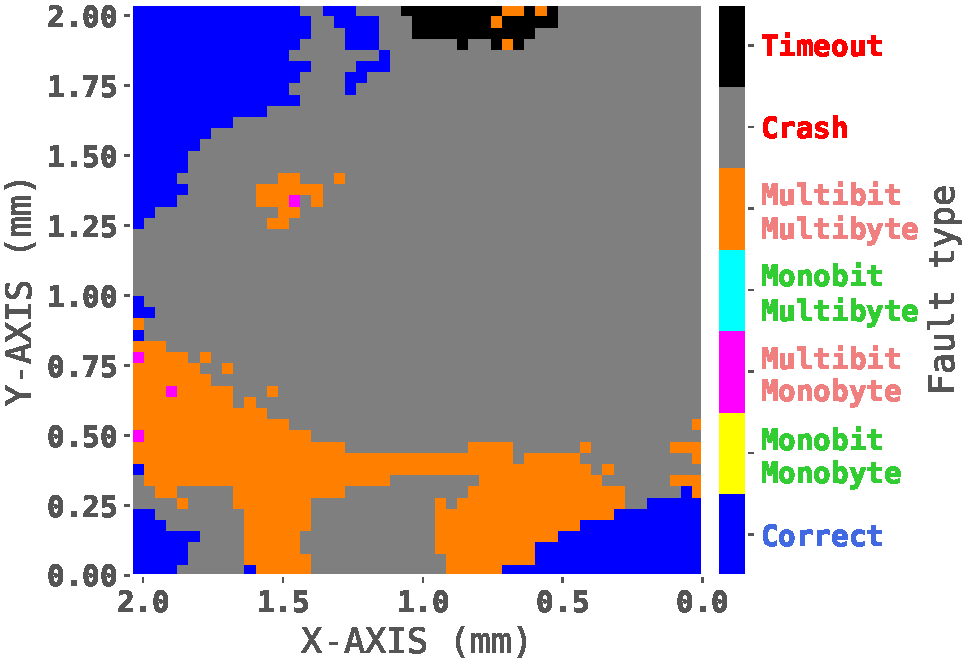
\includegraphics[width=0.995\columnwidth]{./figures/aesFastGndOnly-cropped.pdf}
		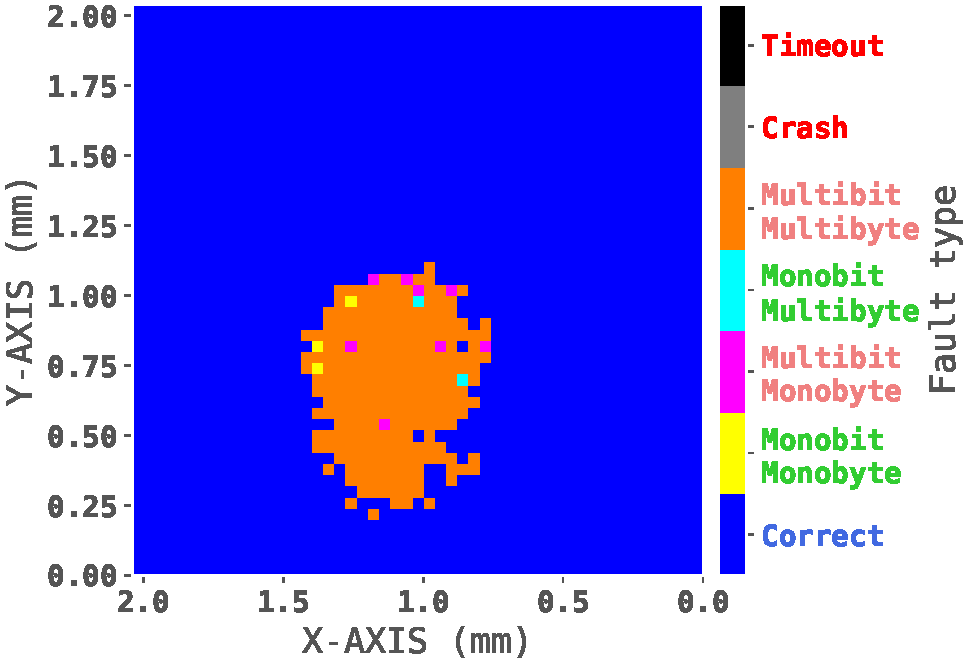
\includegraphics[width=1.0\columnwidth]{./figures/aesFastImpGnd-cropped.pdf}
	\caption{Giraud's attack preliminary FAM}
	\label{giraud_fam}
\end{figure}

			Fig. \ref{giraud_fam} presents the FAM results for both a typical (top) and an improved (bottom) platform.
			The mapped area encloses a little more than the actual AES location, to be sure to map its entirety.

			Let us look at Fig. \ref{giraud_fam} (top) first.
			What is interesting here is that we can spot numerous location where the circuit crashed.
			More specifically, they represent 70 \% of the mapped area.
			This behavior is problematic in such an experiment as it cannot lead to any useful data for a DFA.
			We first thought that the experimental parameters were at fault, so we reiterated the experiment using various different set of parameters, only to observe a majority of crashed locations, while never observing any single bit fault.
%			Despite trying various experimental parameters, we could not observe single bit faults using this setup.
%			However, multibit multibyte faults were easily observed, which was to be expected as they are easy to perform without much effort.

			Then, let us discuss Fig. \ref{giraud_fam} (bottom).
			The first interesting thing to remark here is the total absence of IC crash.
			It is a desirable behavior as it indicates that we did not set a too high voltage or a too long pulse.
			Then, concerning single bit faults, we can spot five locations.
			It is a good sign for a preliminary experiment as it indicates the feasibility of such faults without much effort.
			However, it does not mean that we can perform the attack on one location with one set of parameters.
			It rather means that we can use these locations as good starting points to perform the DFA.

		\subsubsection{DFA results}
			To perform the DFA, we focused on the five previously found monobit locations above the AES core.
			Then, for each location, we used the following parameters:
			\begin{itemize}
				\item Voltage ranging from -300 V to -600 V;
				\item Pulse width ranging from 4.5 ns to 5.5 ns;
				\item Injection delay ranging from \textpm 10 ns around the penultimate AES round.
			\end{itemize}
			For each set of experimental parameters, we had to set some limits when trying to inject faults.
			Indeed, it is required to create a finite and of reasonable length experiment.
			The first limit consists in trying to retrieve a maximum of 100 single bit faults.
			We have chosen this value as it is far more than what is suggested by Giraud's DFA \cite{giraudDfa} description.
			However, if reaching this limit can be easy on some sets of location and parameters, on others, it is almost impossible.
			Therefore, we have set another limit of 10000 trials to achieve the previous goal.
			% !TeX spellcheck = en_US
% !TeX root = ./0_article.tex

\begin{table*}[ht]
	\centering
	\begin{tabularx}{\textwidth}{XXXXXXXXXXXXXXXXX}
		\#B & 0 & 1 & 2 & 3 & 4 & 5 & 6 & 7 & 8 & 9 & 10 & 11 & 12 & 13 & 14 & 15 \\ \hline
		K10 & 0xFF & 0x1F & \cellcolor{red!25}0x42 & 0xE8 & 0xEF & \cellcolor{red!25}0x44 & 0xA5 & 0x6A & 0xCA & 0xE7 & 0x55 & 0x3C & 0xFD & 0x65 & 0x39 & 0x26 \\
		KEY & 0x01 & 0x23 & 0x45 & 0x67 & 0x89 & 0xAB & 0xCD & 0xEF & 0xDE & 0xAD & 0xBE & 0xEF & 0x12 & 0x34 & 0x43 & 0x21
	\end{tabularx}
	\caption{Giraud DFA}
	\label{table_giraud}
\end{table*}

			Thanks to this experiment, we retrieved, using the five previously identified locations, 14 bytes out of 16 of the AES K10 key, which is directly linked to the secret key in an AES-128 bits implementation, as shown in Table \ref{table_giraud}.
			We could not retrieve with the Giraud's DFA the bytes number 2 and 5, which are located in the red cells in the previous table.
			To retrieve the key in its entirety, we performed a brute force method consisting in calculating every possibility for the remaining two bytes.
			Considering a slow laptop being able to compute approximately $10 \cdot 10^3$ AES encryptions per second, and the 16 remaining bits representing 65536 combinations, we decided to blindly calculate every combination.
			This calculation represents around 6.5 seconds of total computation time, and the results are shown in Table \ref{table_giraud}.

%	Three main flaws lie in the platform in its current state:
%	\begin{itemize}
%		\item The pulse generator
%	\end{itemize}

	% !TeX spellcheck = en_US
% !TeX root = ./0_article.tex

\section{Modeling and simulating BBI}
\IEEEPARstart{S}{imulating} a fault injection method behavior is an important part in understanding its mechanisms.
Whether it is EMFI, LFI or BBI, it allows to predict and understand the underlying phenomena at work to set up reliable experiments.
In this paper, we are focusing solely on BBI.

Ideally, we would want to directly observe signals inside integrated circuits, allowing for fine measurements of power supply voltages, logic levels and power current not to cite every physical quantity.
However, embedding sensors into an already existing IC is not possible, and doing so on future IC is costly and takes time to fully implement.
In addition to this, we do not have any guarantee that these sensors will not be disturbed too much by the fault injection.
Therefore, we have decided to take the following approach:
\begin{center}
	Simulation \textrightarrow\ Conclusions \textrightarrow\ Verification
\end{center}

By doing so, we have freed ourselves from hardware limitations.
However, other limitations remains.
Indeed, modern ICs, even the smallest, embed millions of transistors, and with current technologies, it is impossible to evaluate with simulations entire circuits at a transistor level.
Therefore, to tackle these limitations, we decided to adopt an hybrid approach, combining transistor-less models and local logic gates simulations.
This approach is a compromise between accuracy and computational cost/time, and allows simulating relatively big circuits under BBI disturbances
Overall, it is similar to what has been done for EMFI in \cite{mathieuEMFI}.
The resulting simulation flow is divided in three consecutive steps:
\begin{itemize}
	\item The simulation of an IC under BBI using a transistor-less model, allowing for a purely electrical analysis;
	\item The extraction of significant disturbed signals from the previous simulation;
	\item The simulation of functional logic gates under BBI thanks to the previously extracted signals.
\end{itemize}

\subsection{An hybrid simulation flow: building the models}
	Building the correct models for the simulation flow pass through multiple steps.
	As the goal of the hybrid flow is to reduce the computational power required to evaluate an IC, it is still important to maintain a certain accuracy concerning the IC physical structure.
	To do so, the models are designed around actual IC implementations.
	The main building blocks of the models are the power supply network, the standard-cells, and the substrate structure.
	In this work, we are only focusing on bulk substrates: specifically dual-well and triple-well substrates.

	\subsubsection{Power supply rails and standard-cell segments}
		% !TeX spellcheck = en_US
% !TeX root = ./0_article.tex
% LABEL AFTER CAPTION WESH GEOFFREY !!
\begin{figure}[h]
	\centering
	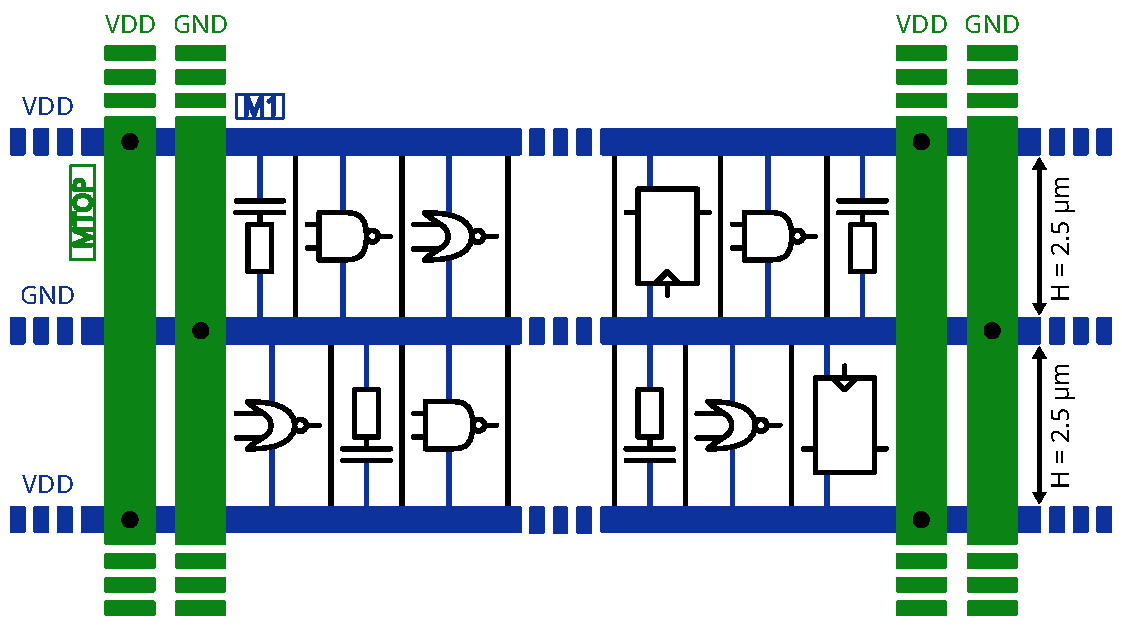
\includegraphics[width=0.49\textwidth]{./figures/psu_std_cell.pdf}
	\caption{A Standard-Cell Segment and its power delivery network.}
	\label{fig_alim_std}
\end{figure}

		The power distribution inside an IC is typically made with a grid-like structure, composed of metal wires stacked on top of each other on planes.
		In each layer, the metal wires are equally spaced and have a dedicated width, which becomes thinner the deeper they are.
		The lowest layer brings the power directly to the transistors.
		Fig. \ref{fig_alim_std} presents a common power delivery network, designed with two metal levels for simplicity.

		Within the metal lines are located standard-cell segments (SCS), composed of decoupling, logic and sequential elements, and are pre-characterized by foundries and categorized depending on their performance (mainly but not exclusively power consumption and speed).
		As illustrated in Fig. \ref{fig_alim_std}, SCS have a constant height, in our case of 2.5 \textmu m, and a variable width depending on how much logic gates each one of them embed.
		As we have stated previously, the hybrid simulation flow use transistor-less models as basic IC building blocks.
		Therefore, the transistors, hence the standard-cell segments, are modeled with passive elements such as resistors and capacitors.

		% !TeX spellcheck = en_US
% !TeX root = ./0_article.tex

\begin{figure}[h]
	\centering
	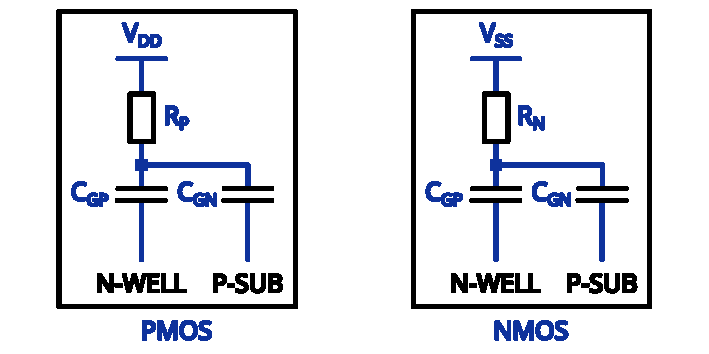
\includegraphics[width=0.9\columnwidth]{./figures/std_cell_logic_passive.pdf}
	\caption{Transistor-less equivalent model of a set of PMOS and NMOS in a SCS.}
	\label{mos_passive}
\end{figure}

		To that end, the elementary SCS chosen measures 30 \textmu m by 5 \textmu m, representing two rows of logic cells.
		This represents about a hundred of logic gates, represented with four resistors and two capacitors, as shown in Fig. \ref{mos_passive}, with half of the transistors conducting, half not conducting.
	%	Respectively, the conducting NMOS and PMOS transistors, whose source is respectively connected to $V_{SS}$ and $V_{DD}$ are respectively equivalent to a passive resistor $R_N$ and $R_P$.
		The conducting NMOS transistors, whose source is connected to $V_{SS}$, are equivalent to the passive resistor $R_N$.
		The conducting PMOS transistors, whose source is connected to $V_{DD}$, are equivalent to the passive resistor $R_P$.
		The resistors values depends on the considered technology, as well as the capacitors values, and can be adjusted and calculated according to one needs.

	\subsubsection{The substrate}
		% !TeX spellcheck = en_US
% !TeX root = ./0_article.tex

\begin{figure}[h]
	\centering
	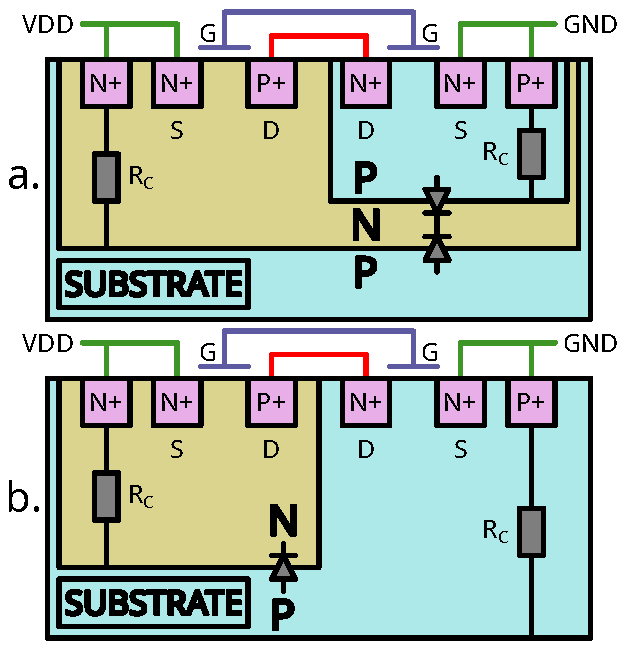
\includegraphics[width=0.35\textwidth]{./figures/substrate_2.pdf}
	\caption{Triple-well (a) and Dual-well (b) inverter cross-sectional view.}
	\label{fig_sub}
\end{figure}

		Because BBI can be performed thanks to the silicon substrate as the main physical environment transferring energy from a generator to an IC, it is fundamental to elaborate a proper substrate model to precisely represent the various involved phenomena.
		As stated previously, our work focuses on bulk substrates, and in most cases, the substrate silicon is P-doped.
		There are two typical ways of lithographing the transistors in a bulk substrate, using dual-well or triple-well structures.
		Dual-well substrates are commonly found in moderately old circuits, while triple-well substrates are found in more recent circuits, while not bleeding-edge.

		To properly understand how the differences between dual-well and triple-well substrates change the resulting model, let us analyze the cross-sectional schematics of an inverter created respectively in a triple-well and a dual-well substrate, as shown respectively in Fig. \ref{fig_sub}.a and Fig. \ref{fig_sub}.b:
		\begin{itemize}
			\item In the triple-well substrate, the NMOS transistors are lithographed into a P-doped silicon well, itself lithographed inside a N-doped well, buried inside the P-doped substrate. The PMOS transistors are located inside the N-doped well;
			\item In the dual-well substrate, the PMOS transistors are still located inside the N-doped well, however, the NMOS are lithographed directly inside the P-doped substrate.
		\end{itemize}
		On the one hand, the triple-well substrate reveals two diodes:
		\begin{itemize}
			\item One formed between the P-well and the N-well;
			\item Another formed between the N-well and the P-substrate.
		\end{itemize}
		On the other hand, the dual-well substrate only reveals one diode between the N-well and the P-substrate.

	\subsubsection{The resulting model}
		Thanks to what we have introduced previously, we can now build the elementary building blocks for our hybrid simulation flow.
		It combines the power delivery network architecture, the equivalent logic gates models, and the substrate structure, all in an embedded model.
		This model represents an elementary section of the simulated IC, measuring 30 \textmu m by 5 \textmu m by $t_{Sub}$ \textmu m, the latter being the substrate thickness, a parameter which will vary depending on each considered IC.
		% !TeX spellcheck = en_US
% !TeX root = ./0_article.tex

\begin{figure*}[ht]
	\centering
	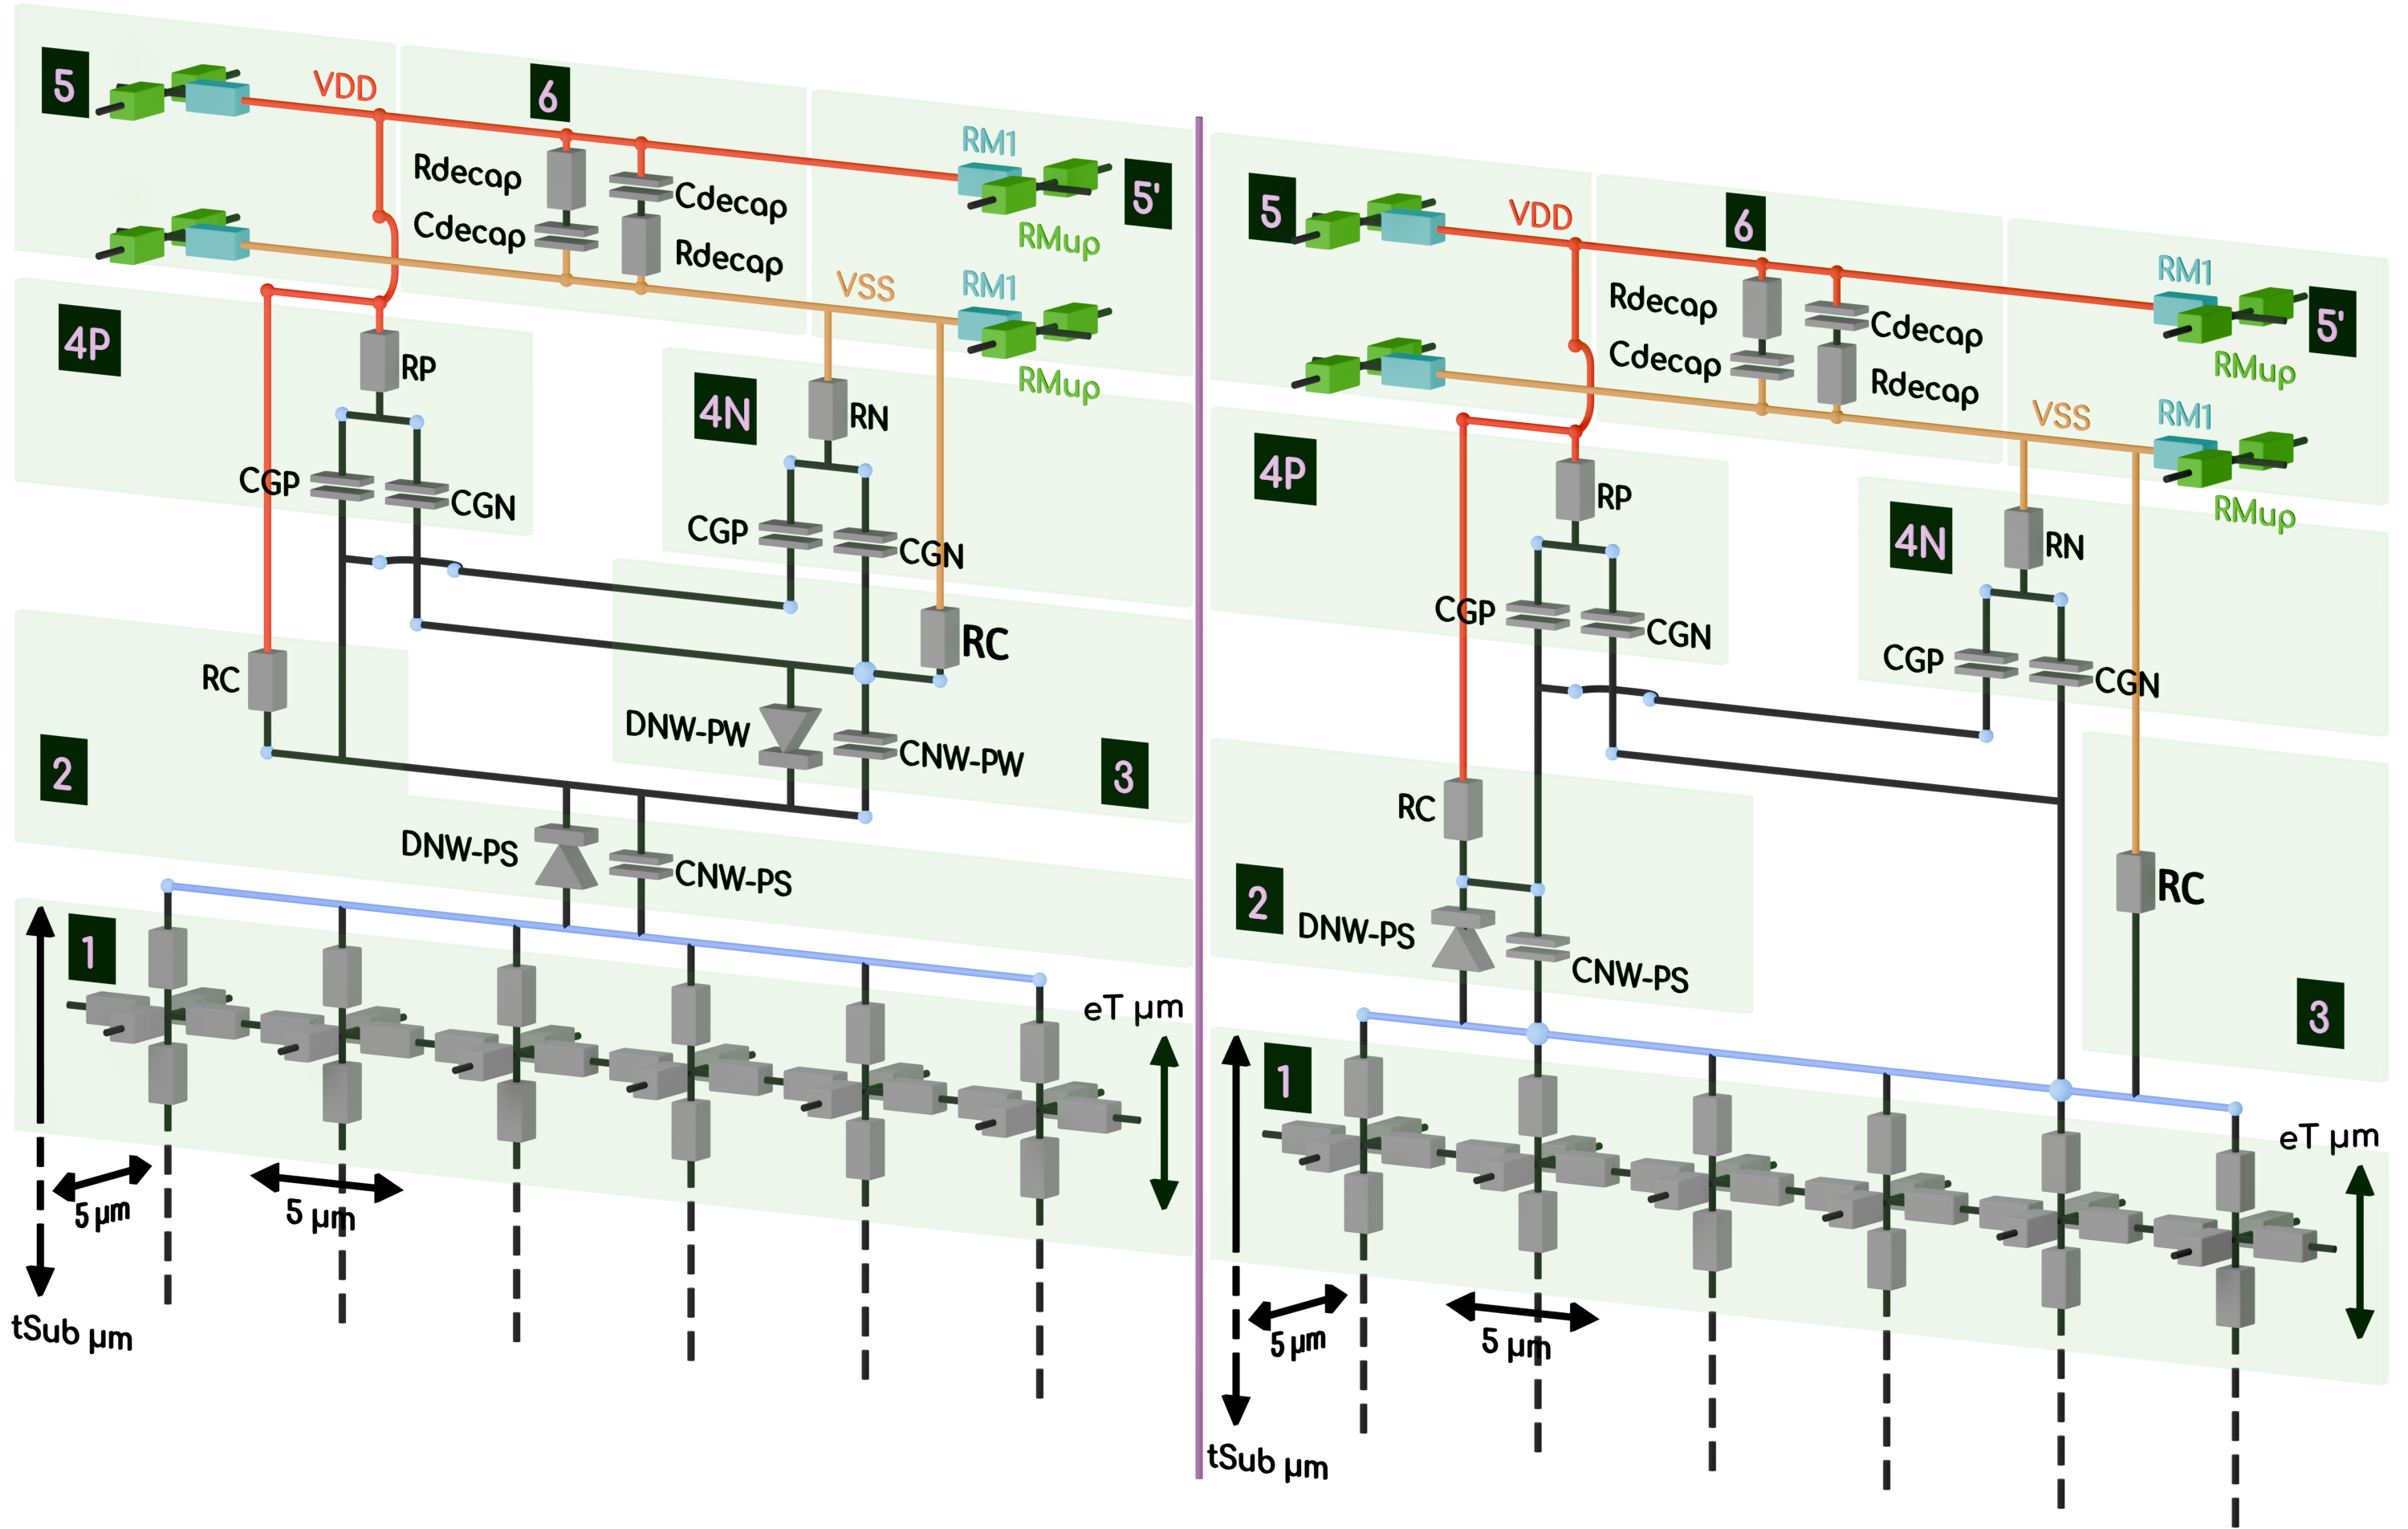
\includegraphics[width=0.95\textwidth]{./figures/dual+triple3.png}
	\caption{Triple well (left) and dual well (right) std cell \textcolor{red}{(PEUT ETRE FAIRE DES SOUS-FIGURES)}}
	\label{fig_triplewellstdcell}
\end{figure*}

		As we consider both triple-well and dual-well substrate, there are two resulting elementary models, shown in Fig. \ref{fig_triplewellstdcell}.
		Each model is composed of various sub-regions, whose descriptions follow:
		\begin{itemize}
			\item \ovalbox{1} is the substrate network, divided into six sub-networks of six resistors for finer details;
			\item \ovalbox{2} is the first P-N silicon junction, common to both models;
			\item \ovalbox{3} is the access resistor (DW) or the second junction (TW);
			\item \ovalbox{4P} is the PMOS equivalent section;
			\item \ovalbox{4N} is the NMOS equivalent section;
			\item \ovalbox{5, 5'} are the power supply metal layers (upper metal in green, first level in blue);
			\item \ovalbox{6} is the power supply decoupling.
		\end{itemize}
		As we have stated before, these models only represent a small portion of the modeled IC.
		To create an entire IC of a defined size, it is required to instantiate and interconnect as much as needed the elementary models.
		By doing so, we can create a bigger model of virtually any size.
		The language we have chosen to work with the simulation is the SPICE language.
		However, we created a custom Python script to interconnect the SCS together and generate a generic SPICE file.

\subsection{An hybrid simulation flow: performing simulations}
	Now that we set up the base models and their duplication, we can perform simulations with those models.
	To properly use these models, it is required, in the first place, to validate them through various steps to ensure their reliability.
	To that end, we generated an IC measuring 600 \textmu m by 600 \textmu m with a 200 \textmu m substrate thickness, and performed an operating point to verify the correctness of the models.
	% !TeX spellcheck = en_US
% !TeX root = ./0_article.tex

\begin{table}[H]
	\label{tab_op}
	\centering
	\begin{tabular}{lll}
		Value  & Triple-well & Dual-well \\ \hline
		$I_{GND}$                               & 2 nA          & 2.2 nA    \\
		$I_{VDD}$                                & -7 nA        & 3 nA        \\
		$\overline{GND_{drop}}$    & 2 nV         & 2 nV        \\
		$\overline{V_{DD_{drop}}}$    & 3 nV         & 3 nV       
	\end{tabular}
	\caption{op point}
\end{table}

	% !TeX spellcheck = en_US
% !TeX root = ./0_article.tex

\section{Effects of BBI on IC operation}
\subsection{Extending the models: logic gates simulation}
	As we have stated previously, it is required, to complete the models, to properly consider the logical behavior of the considered circuits, which allows for a better appreciation of BBI induced effects and their consequences.
	These additional steps consist in modeling actual logic and sequential elements in the same or in a close technology as the considered IC, while extracting the significant disturbed signals from the SCS simulation and injecting them into these logic devices.
	For this purpose, split this section into two subsections:
	\begin{itemize}
		\item A first section dedicated to studying a static logic gate: the classical inverter;
		\item A second section dedicated to studying a sequential element: the DFF.
	\end{itemize}

\subsection{BBI effects on static logic gates: inverters}
	% !TeX spellcheck = en_US
% !TeX root = ./0_article.tex

\begin{figure}[h]
	\label{ivxbufmos}
	\centering
	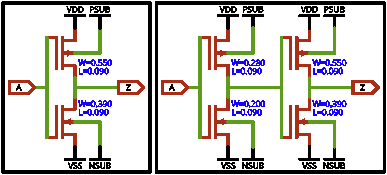
\includegraphics[width=0.5\textwidth]{./figures/IVX_BUFF_X4_3.pdf}
	\caption{IVX MOS SCH \textcolor{red}{A-T-ON LE DROIT DE METTRE CE SCHÉMA ?}}
\end{figure}

	Because inverters can have two stable output states, we will consider two cases for each substrate scenario: a normally high inverter (Fig. \ref{ivxbufmos}.a) and a normally low inverter (Fig. \ref{ivxbufmos}.b).
%		 as it is illustrated on the model shown in Fig. \ref{ivxbufmos}: a normally high and a normally low inverter.
	The inverters are connected to four external signals which are extracted from the previous SCS simulation:
	\begin{itemize}
			\item VDD: the power supply voltage;
			\item VSS: the power supply reference voltage;
			\item PSUB: the bulk voltage of the PMOS transistors;
			\item NSUB: the bulk voltage of the NMOS transistors.
		\end{itemize}
	The voltages PSUB and NSUB depend on the substrate type.
	On the one hand, in the dual-well scenario, NSUB is connected to the epitaxial layer, while PSUB is connected to the N-well.
	On the other hand, in the triple-well scenario, NSUB is connected to the P-well and PSUB to the N-well.

	All of this gives us four scenarios	 to study.
	For clarity and because two of the four scenario are less noteworthy, we will only talk about two of them:
	\begin{itemize}
		\item The triple-well substrate and the normally high inverter;
		\item The dual-well substrate and the normally low inverter.
	\end{itemize}
	Then, for each scenario, we will analyze seven signals of interest:
	\begin{itemize}
		\item The backside voltage pulse, for reference purposes;
		\item The local differential power supply voltage;
		\item The current sum of the inverter;
		\item The inverter load current;
		\item The inverter output;
		\item The NSUB voltage;
		\item the PSUB voltage.
	\end{itemize}
	The signals extracted from the SCS simulations come from the standard-cell located directly below the BBI probe, a.k.a the cell targeted by the injection.
	% !TeX spellcheck = en_US
% !TeX root = ./0_article.tex

\begin{figure}[h]
	\centering
%	\vspace{\vsp mm}
	\subfloat[][Dual-well]{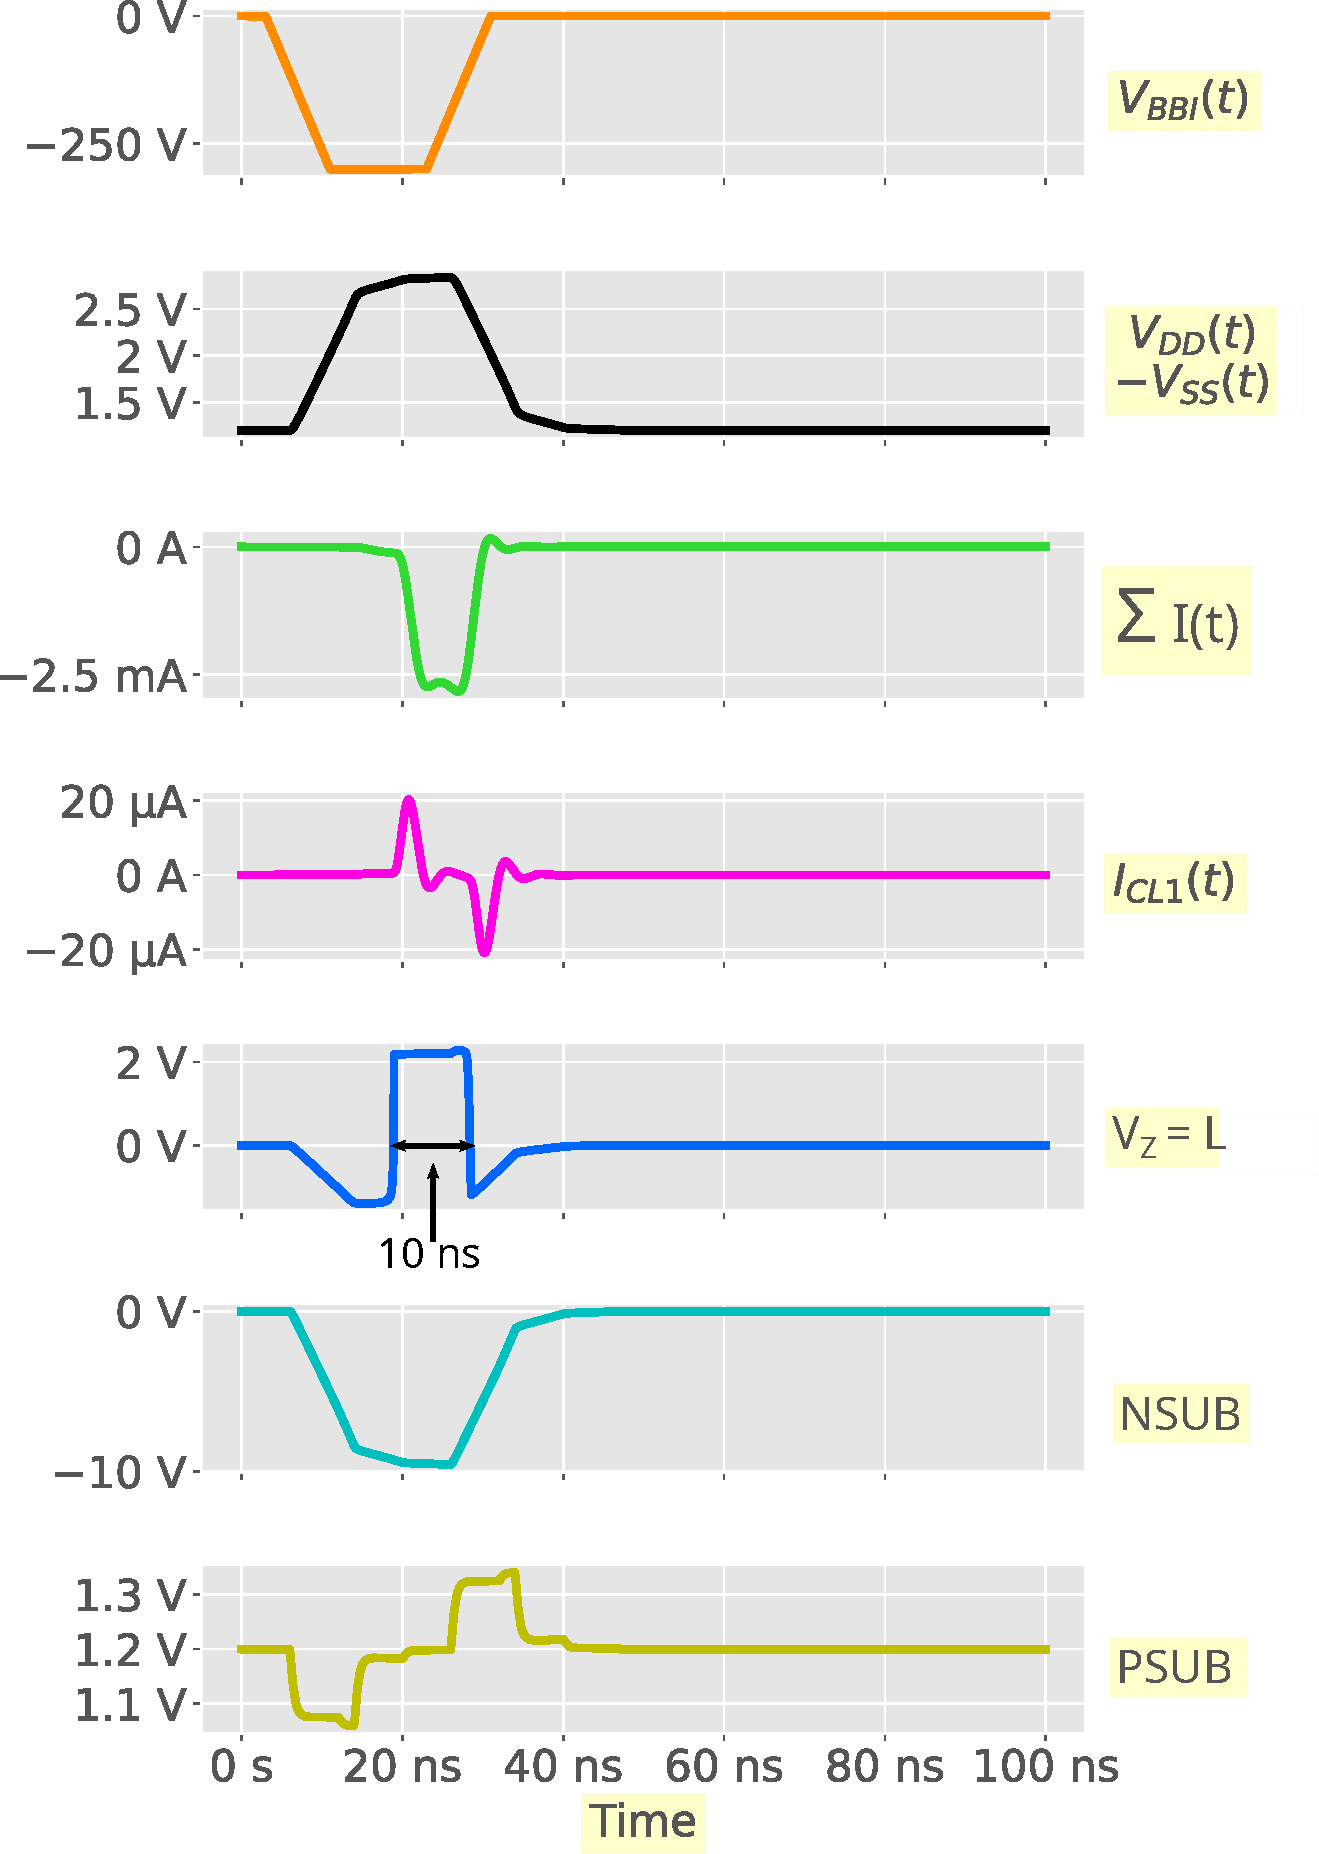
\includegraphics[width=0.506\columnwidth]{./figures/logic_gates_solo_M0_DW.pdf}}
	\subfloat[][Triple-well]{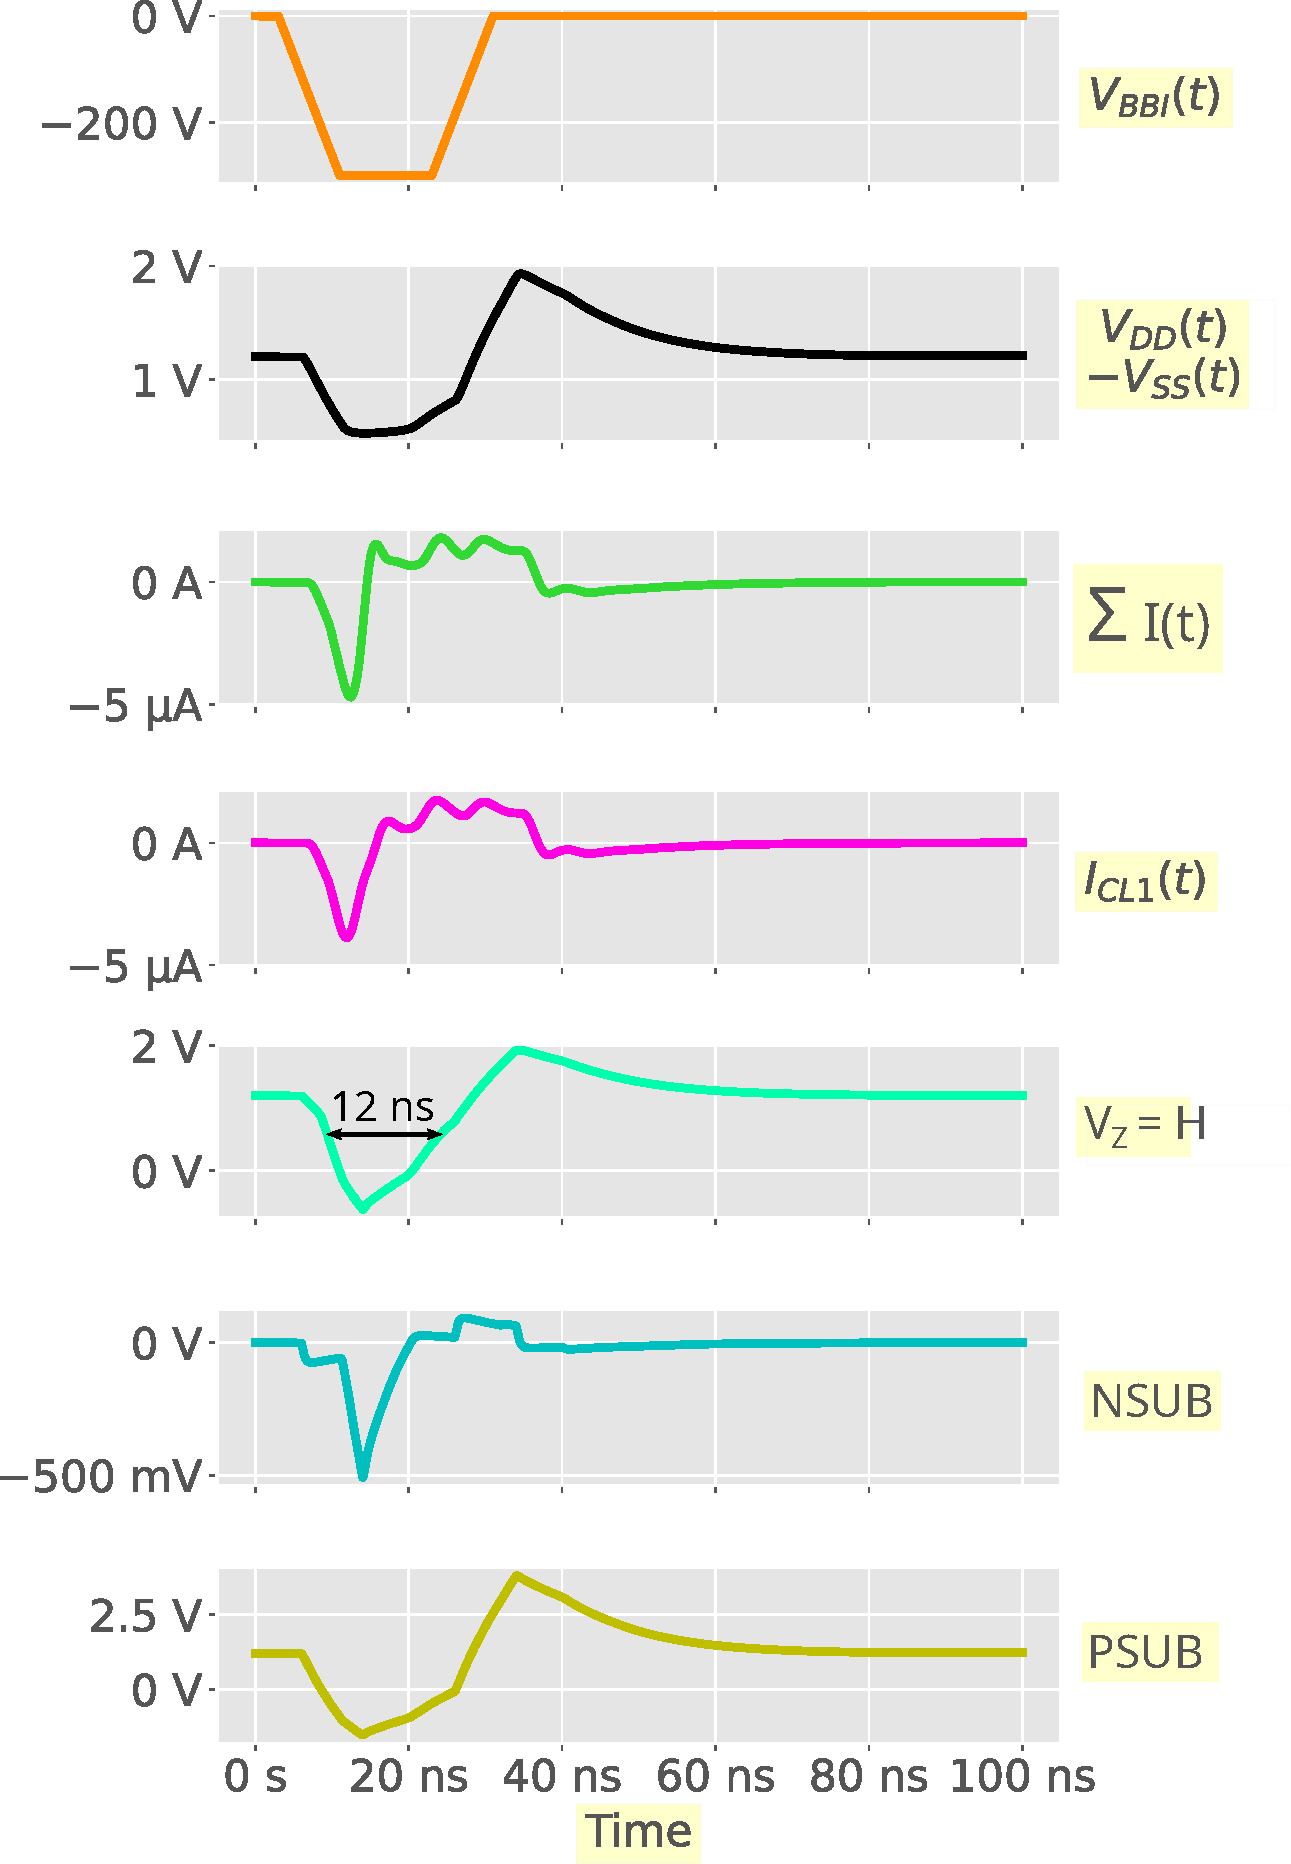
\includegraphics[width=0.494\columnwidth]{./figures/logic_gates_solo_M0_TW.pdf}}
	\caption{Inverters simulation results}
	\label{ivxsimu}
\end{figure}

	Fig. \ref{ivxsimu} presents the inverter simulation results for both considered scenarios.

	First, let us focus on the dual-well inverter.
	The corresponding schematic is shown in Fig. \ref{ivxbufmos}b, and the simulation results are shown in Fig. \ref{ivxsimu}a.
	In that case, as we have seen before, the global IC coupling is resistive, with a discrepancy between VSS and VDD.
	Therefore, the inverter current sum (green) follows a DC-response, similar to the differential power delivery voltage (black).
	The inverter output follows the current sum curve, and its output goes from a low to a high logic value during 10 ns, then back to its original state.
	It is further corroborated by looking at the load current, which is charged on the first pulse edge, then discharged on the second one.

	Second, concerning the triple-well inverter, where the results are shown in Fig. \ref{ivxsimu}b and the schematic in Fig. \ref{ivxbufmos}a, the substrate is globally AC-coupled.
	It can be seen on the current sum curve, which follows almost exactly the capacitive load current curve.
	The inverter output, for its part, is discharged like the load, and goes from a high logic value to a low value during 12 ns before returning to its original value.

	These observations are of great value because we can discuss a fault model for BBI, similar to what has been studied for EMFI and LFI.
	The previous results seem to indicate that the faults created using BBI are data-dependent.
	Indeed, if we lower the voltage of an inverter outputting a low value, or the opposite, it has theoretically no direct effect on the logic value.
	However, we have seen that it is possible, depending on the substrate type, to observe bit set or reset.
	Eventually, thanks to these results and the previous ones regarding current density in the substrate in Fig. \ref{sim_res_dw_neg}, \ref{sim_res_dw_pos}, \ref{sim_res_tw_neg} and \ref{sim_res_tw_pos}, it seems that BBI effects are local.

\subsection{BBI effects on dynamic logic gates: DFF}
	% !TeX spellcheck = en_US
% !TeX root = ./0_article.tex

\begin{figure}[h]
	\centering
	%	\vspace{\vsp mm}
	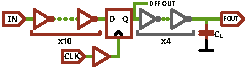
\includegraphics[width=\columnwidth]{./figures/dff_ivx_chain_3.pdf}
	\caption{DFF chain}
	\label{dffchain}
\end{figure}

	Now that we have analyzed the behavior of static inverters, it is important to consider studying the behavior of sequential elements such as a very common one: the D Flip-Flop.
	These devices are used in every IC as an elementary memory element to sample data manipulated by the combinatorial logic.
	To test the DFF behavior under BBI, we placed it in the middle of a logic path and buffered its clock.
	The goal of this simulation is to mix the behavior of a disturbed logic path outputting to a disturbed DFF, outputting to a non-disturbed logic path.
	The non-disturbed path is here to mimic the behavior of far away logic gates receiving disturbed data while having a correct power supply.
	
	Similar to what we have done in the previous section, we will extract signals from the SCS simulation and inject them into this test circuit.
	The simplified schematic of this circuit is shown in Fig. \ref{dffchain}.
	The first ten inverters, the buffer and the DFF are disturbed, while the four last inverters are not disturbed.
	The load $C_L$ mimics another set of logic gates which are loaded into the four inverters.
	As we did with the inverters, we will only consider negative pulses, both for a dual-well and a triple-well substrate.
	% !TeX spellcheck = en_US
% !TeX root = ./0_article.tex

\begin{figure}[h]
	\centering
	%	\vspace{\vsp mm}
	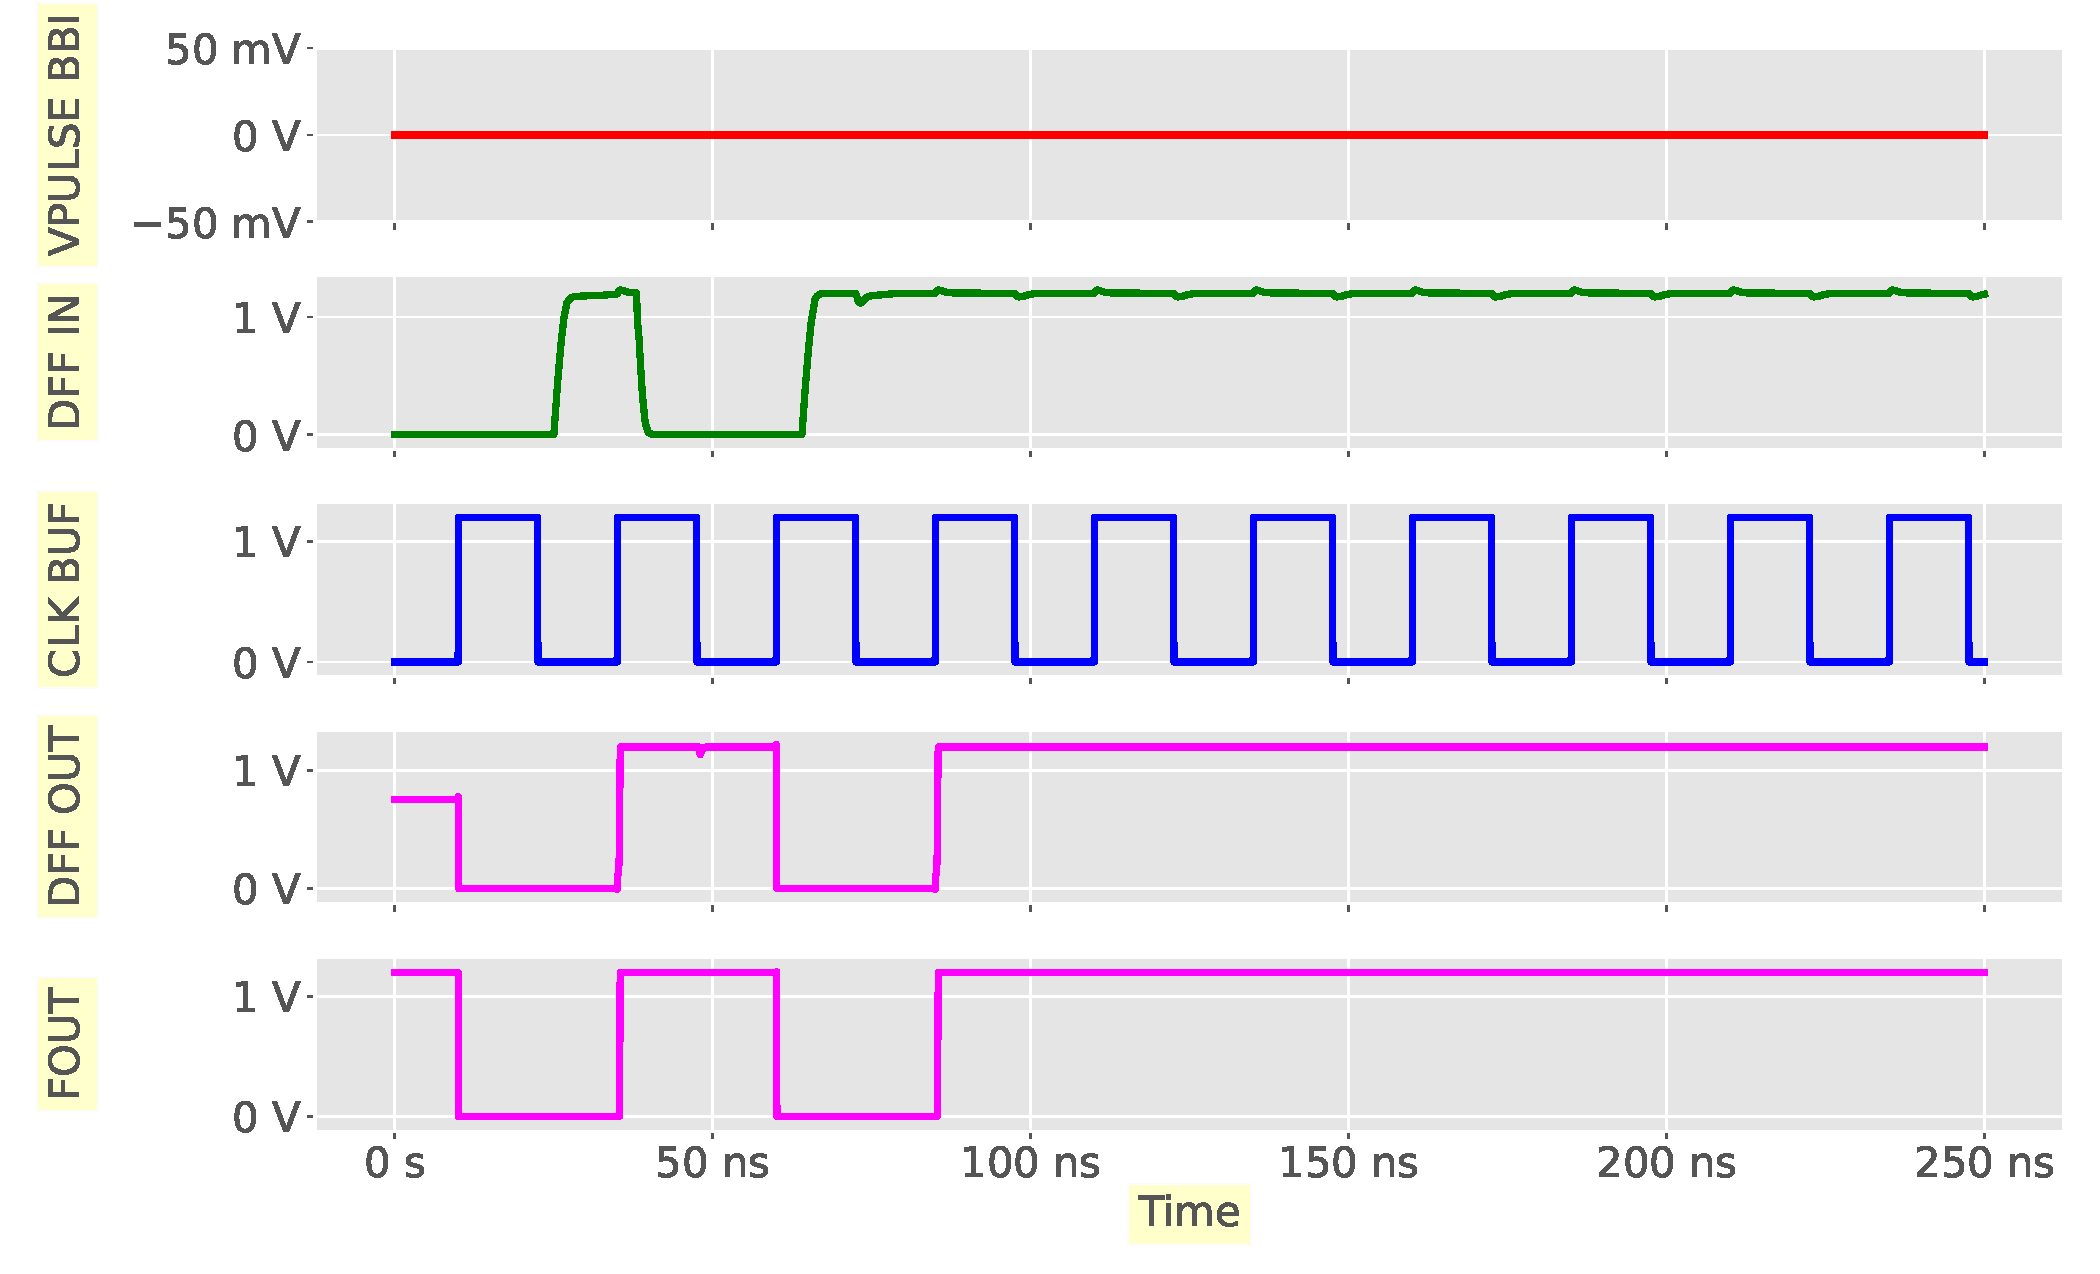
\includegraphics[width=\columnwidth]{./figures/anim0000-cropped.pdf}
	\caption{DFF path: idling}
	\label{dffidle}
\end{figure}

	Before diving into the simulation results, let us analyze what would be the normal behavior of the considered DFF.
	Fig. \ref{dffidle} presents the normal behavior of the modeled DFF path.
	The flip-flop is governed by a 40 MHz clock, and we perform three write operations with alternating logic levels (H \textrightarrow\ L \textrightarrow\ H), to finally let it rest at the last logic level.
	Because a DFF is a dynamic device, there are many interesting moments to observe depending on when the voltage pulse is injected.
	Therefore, we cannot represent every noteworthy moment, so we have chosen the most interesting according to us.
	First, we will analyze results where the injections are performed during the steady state of the DFF chain,
	Then, we will analyze the DFF behavior during the write operations.
%	During these simulations, we initialize the DFF with a low logic level, then a 
	
	\subsubsection{Dual-well substrate, negative pulse}
		% !TeX spellcheck = en_US
% !TeX root = ./0_article.tex

\begin{figure}[h]
	\centering
	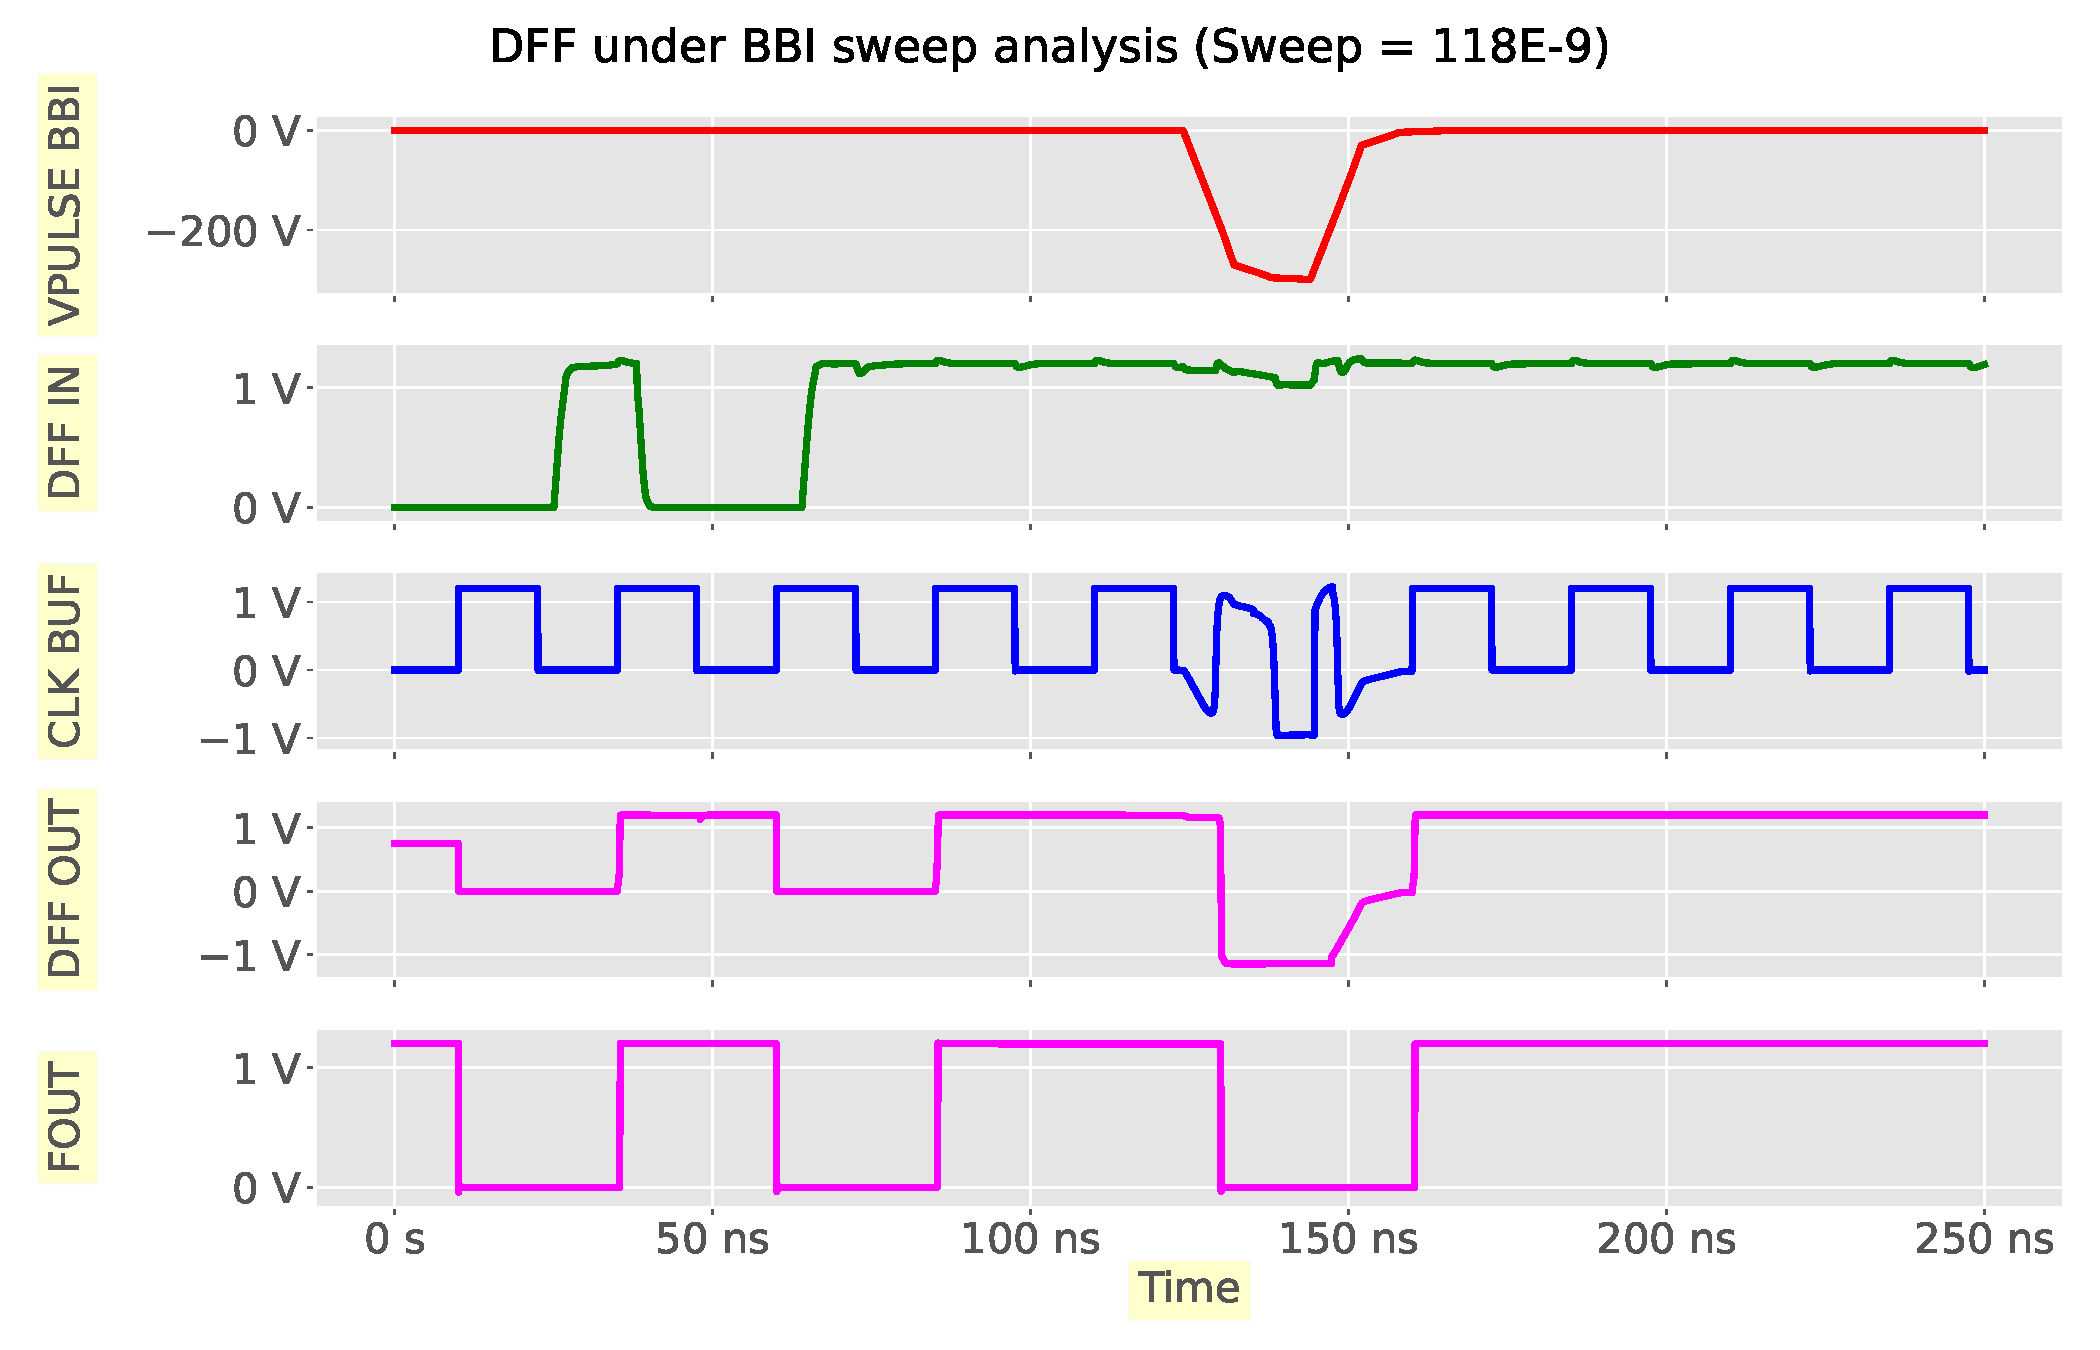
\includegraphics[width=\columnwidth]{./figures/dff-pdf-dw-neg/anim0108.pdf}
	\caption{DFF static DW}
	\label{dffstatic-dw}
\end{figure}

		Fig. \ref{dffstatic-dw} shows the simulation results for a dual-well negative pulse for a steady state disturbed DFF.
		Five signals are represented in this order, allowing us to get insights on the circuit behavior:
		\begin{itemize}
			\item The BBI voltage pulse for reference;
			\item The DFF input signal;
			\item The buffered DFF clock;
			\item The DFF output;
			\item The four last inverters output;
		\end{itemize}
		The results show that the DFF input is not disturbed enough to trigger a logic value change.
		However, the DFF output drops down to -1 V, similar to its own buffered clock.
		This voltage drop, lasting for 25 ns, reverberates on the clean inverters output, resulting in a low logical value being output.
		In addition to this, the disturbances on the clock shows the creation of two parasitic clock pulses, replacing a normal one during the injection.
		
		% !TeX spellcheck = en_US
% !TeX root = ./0_article.tex

\begin{figure}[h]
	\centering
	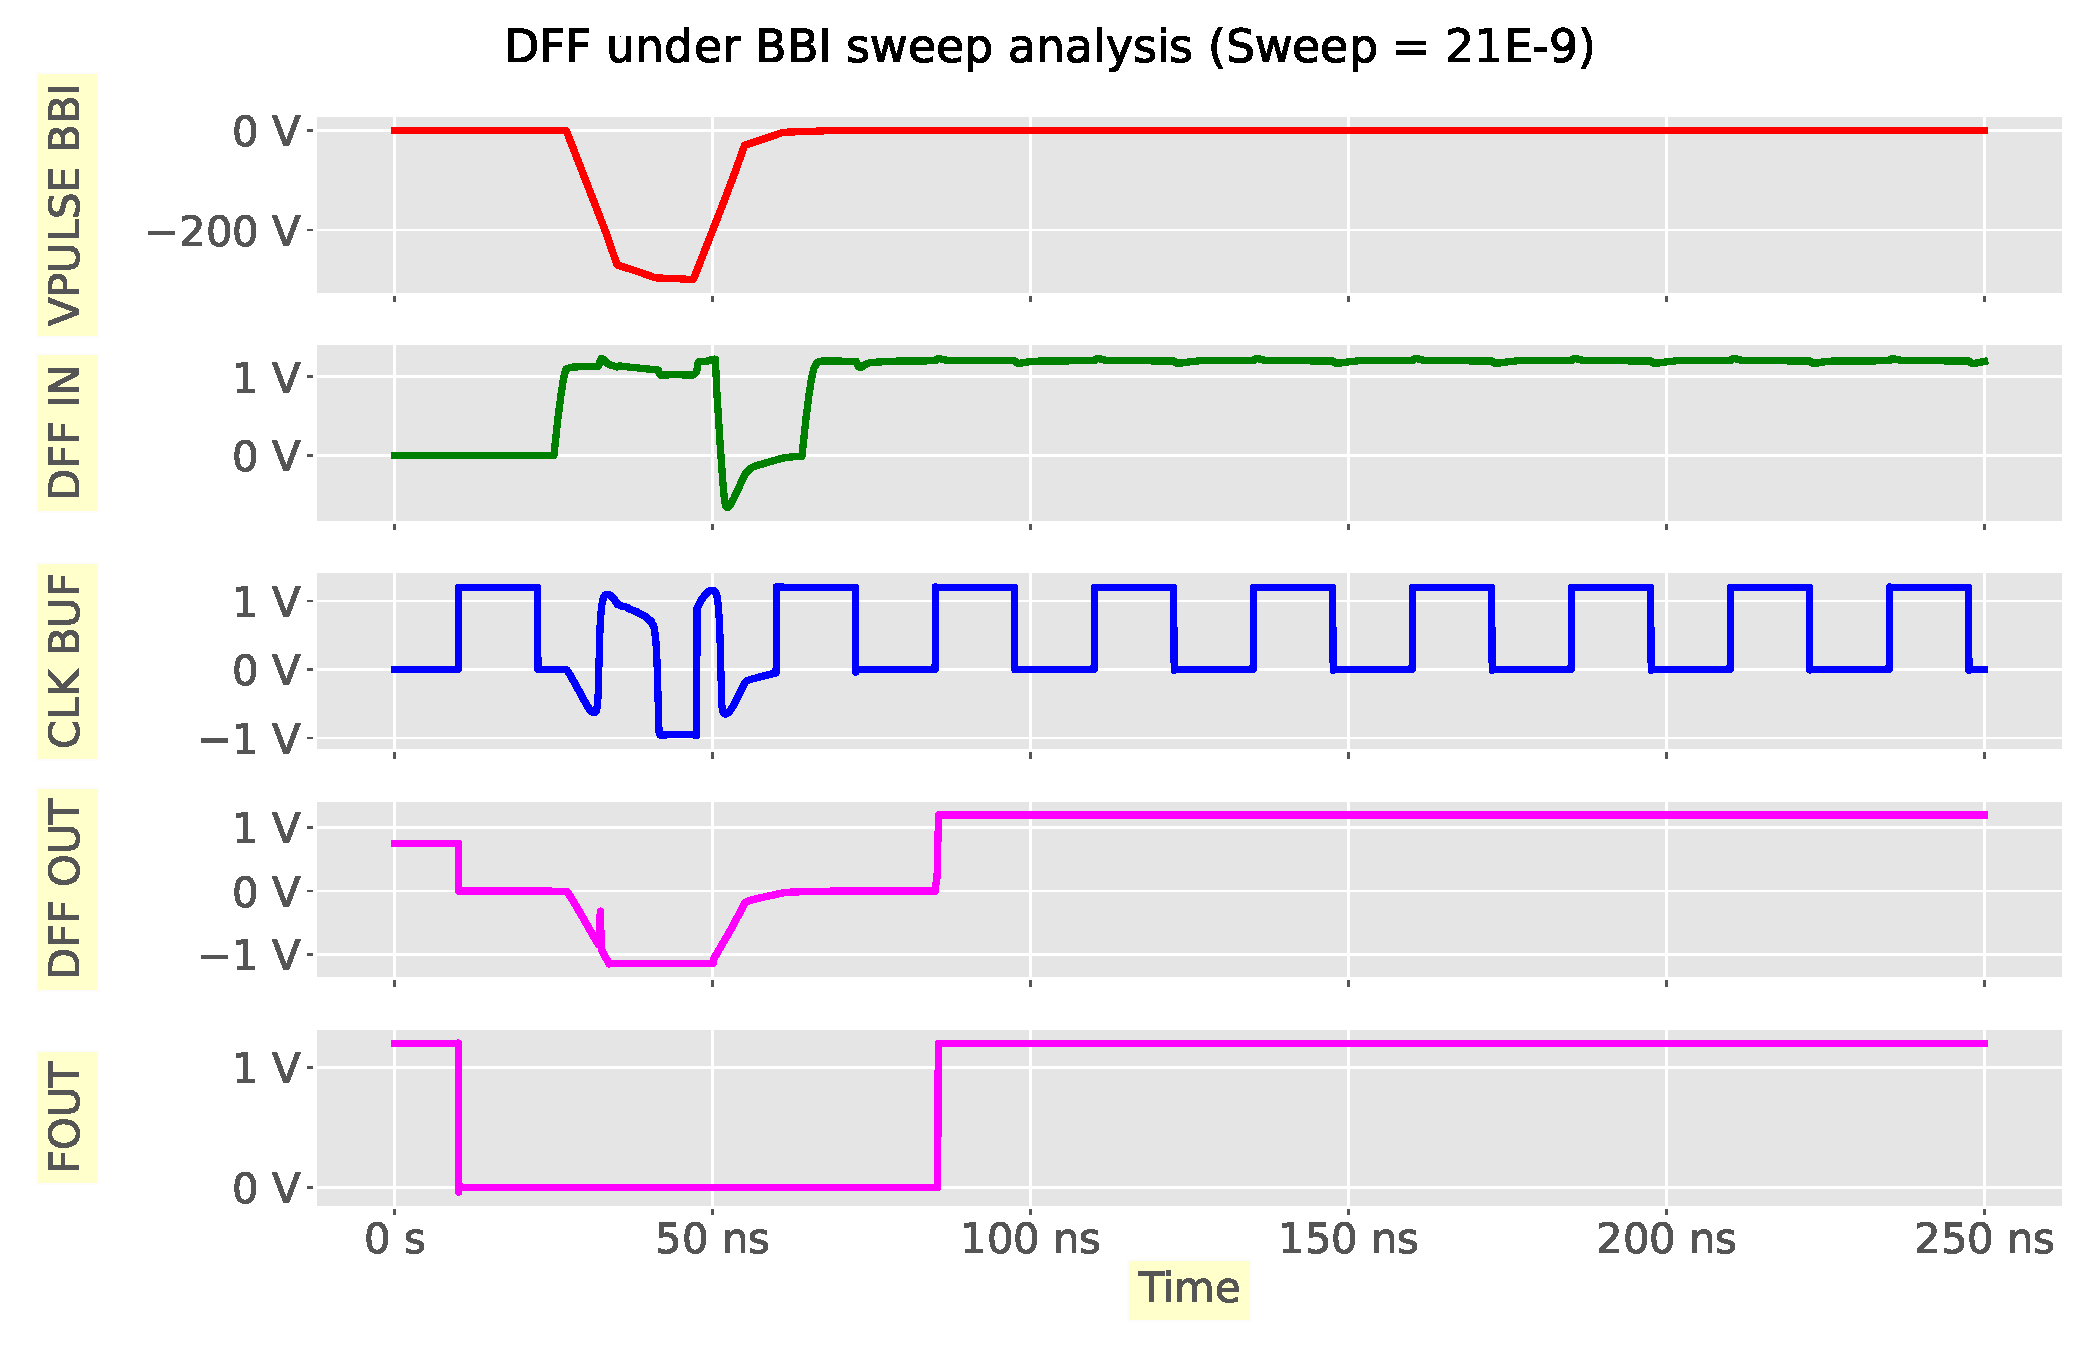
\includegraphics[width=\columnwidth]{./figures/dff-pdf-dw-neg/anim0011.pdf}
	\caption{DFF path: dynamic dual-well}
	\label{dffdynamic-dw}
\end{figure}

		Then, Fig. \ref{dffdynamic-dw} shows the exact same scenario with a different injection time, performed during the first write operations.
		These results show that the disturbances prevent the second write operation, supposed to write a high logic value in the DFF.
		Therefore, this data will never be sampled by the DFF and therefore will never propagate to the output of the circuit.
	
	\subsubsection{Triple-well substrate, negative pulse}
		% !TeX spellcheck = en_US
% !TeX root = ./0_article.tex

\begin{figure}[h]
	\centering
	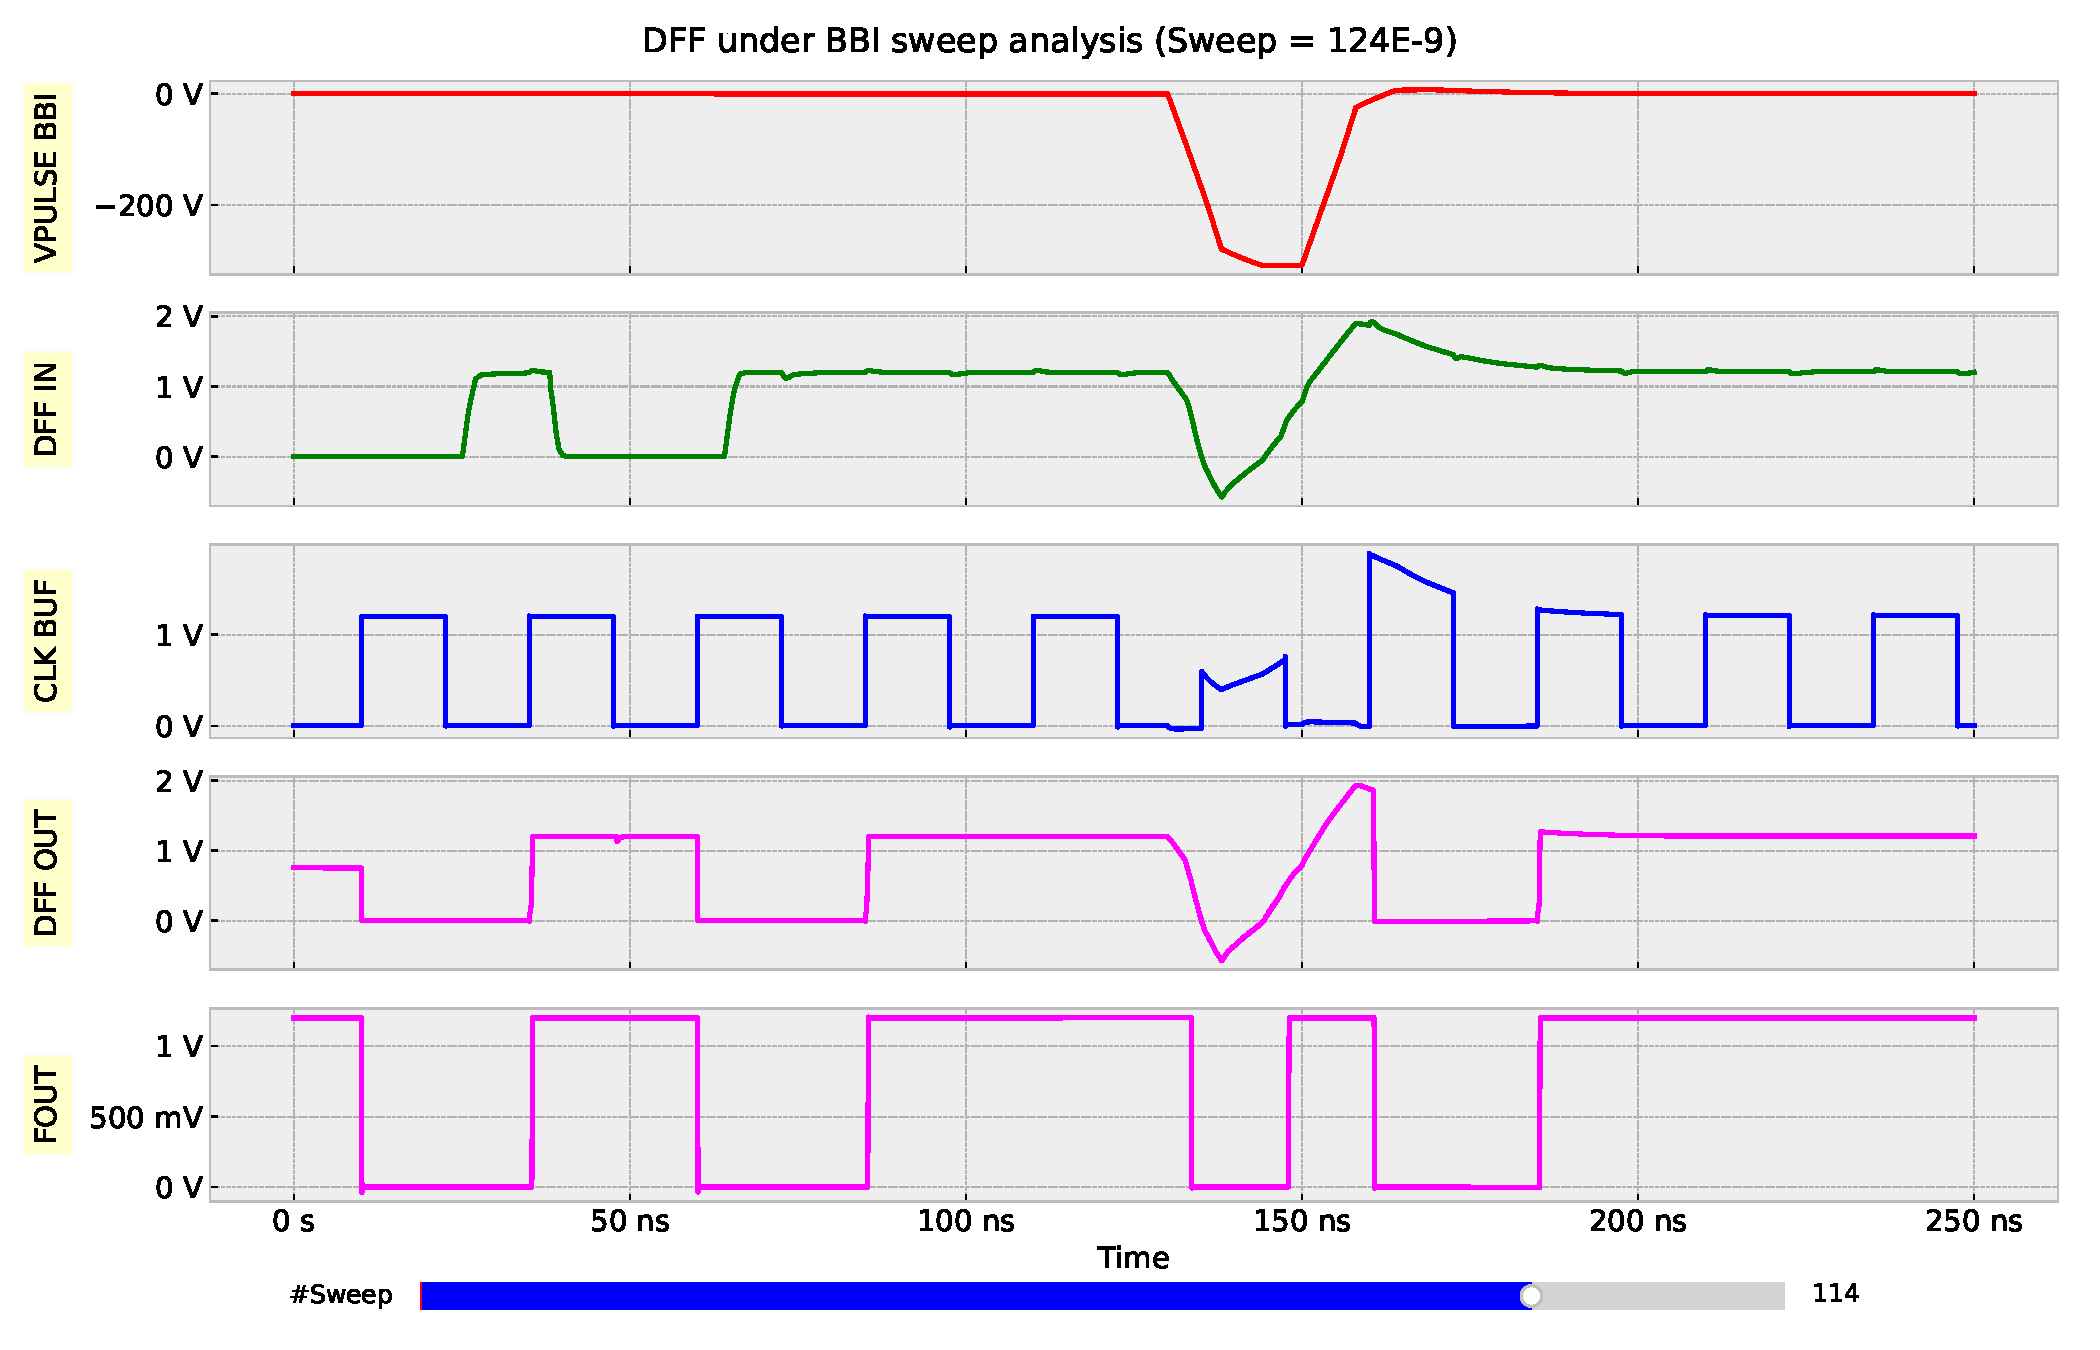
\includegraphics[width=\columnwidth]{./figures/dff-pdf-tw-neg/anim0114.pdf}
	\caption{DFF path: static triple-well}
	\label{dffstatic-tw}
\end{figure}

		Fig. \ref{dffstatic-tw} shows the simulation results for a triple-well negative pulse for a steady state disturbed DFF.
		
	\textcolor{orange}{The rest of this section is in the making. Some experiments are missing to illustrate the DFF results. We are waiting for the newly opened circuits.}

%	For this purpose, we modeled an inverter, a buffer and a DFF.
%	The inverter and the buffer schematics, alongside their transistors sizes, are shown in Fig. \ref{ivxbufmos}.
%%	% !TeX spellcheck = en_US
% !TeX root = ./0_article.tex

\begin{figure}[h]
	\label{dffmos}
	\center
	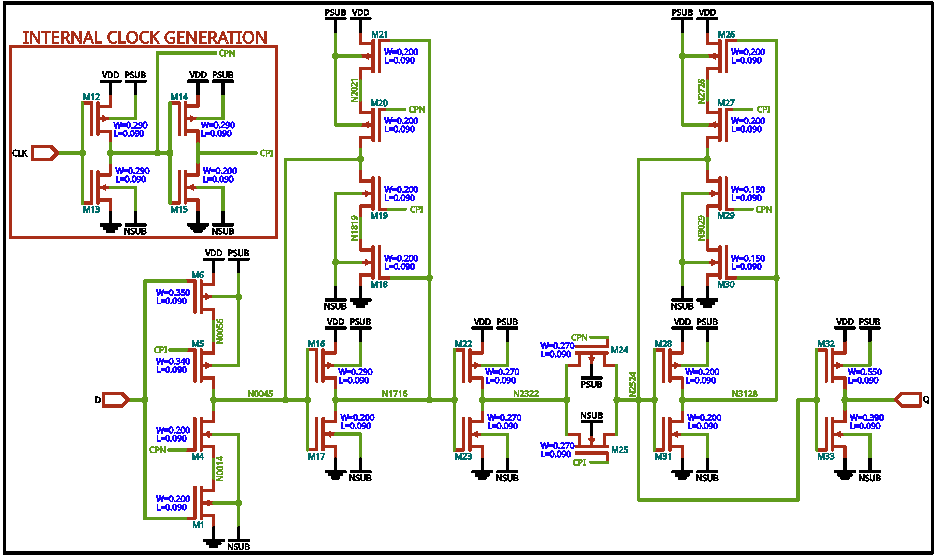
\includegraphics[width=0.5\textwidth]{./figures/CORE65GPSVT_HS65_GS_DFPQX4.pdf}
	\caption{DFF MOS SCH \textcolor{red}{A-T-ON LE DROIT DE METTRE CE SCHÉMA ?}}
\end{figure}

%%	The complete DFF schematic is shown in Fig. \ref{dffmos}.
%
%	Each logic element is connected to four external signals:
%%	The significant extracted signals are the following:
%	\begin{itemize}
%		\item VDD: the power supply voltage;
%		\item VSS: the power supply reference voltage;
%		\item PSUB: the bulk voltage of the PMOS transistors;
%		\item NSUB: the bulk voltage of the NMOS transistors.
%	\end{itemize}
%	These are the signals which are extracted from the SCS simulations.
%	The voltages PSUB and NSUB depend on the substrate type.
%	On the one hand, in the dual-well scenario, NSUB is connected to the epitaxial layer, while PSUB is connected to the N-well.
%	On the other hand, in the triple-well scenario, NSUB is connected to the P-well and PSUB to the N-well.
%	% !TeX spellcheck = en_US
% !TeX root = ./0_article.tex

\begin{figure}[h]
	\label{dffChain}
	\centering
	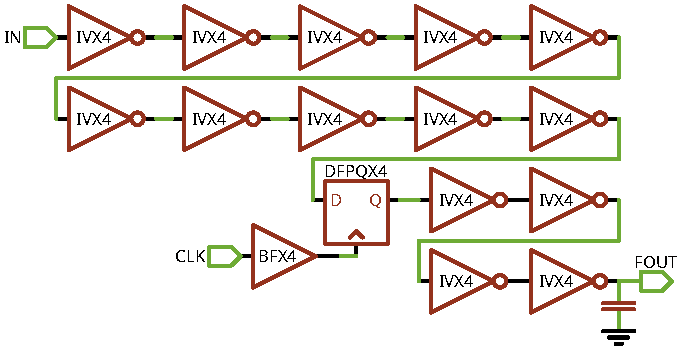
\includegraphics[width=0.5\textwidth]{./figures/dff_ivx_chain_2.pdf}
	\caption{DFFCHAIN}
\end{figure}

%	The resulting simulated logic circuit, combining several inverters, a buffer and a DFF, is shown in Fig. \ref{dffChain}.
%	The first ten inverters, the buffer and the DFF are disturbed thanks to the extracted signals.
%	The four last inverter are not disturbed and are powered with ideal power signals.
%	Their role is to mimic a distant logic block receiving the DFF "BBI disturbed" logic signals.
%	The simulations are performed, as previously, for both a dual-well scenario and a triple-well scenario.
%	However, and for simplicity showing the results, we did not consider the positive pulse case, as we observed high level of destructiveness on actual ICs.
%
%	Presenting such results on a logic path embedding a DFF on a digital or physical static medium is not an easy task.
%	Therefore, we have chosen some specific time during the simulation where we think the results are noteworthy.
%	However, every simulation step is useful to some extent.
%	Therefore, we provide additional simulation results in our GitHub repository dedicated to this paper (\textcolor{red}{mettre repo ?}).

	% !TeX spellcheck = en_US
% !TeX root = ./0_article.tex

\section{Conclusion}
	\IEEEPARstart{B}{ody} biasing injection has seen a re-emergence since 2020 \cite{bbiColin}, and various works have brought more and more knowledge throughout the years.
	BBI, contrary to EMFI or LFI, uses the silicon substrate of as the main physical medium to interact, transfer energy, and disturb integrated circuits.
	We introduced, through this work, the cumulative knowledge we gathered concerning BBI.
	This involves various aspects of the subjects.

	First, we studied better methods to improve BBI experiments repeatability and reliability through low-cost platform modifications.
	We supported these results with actual experiments such as Fault Analysis Mappings and a Differential Fault Attack.

	Then, we introduced large-scale IC modeling thanks to the use of transistor-less models allowing to reduce the computational power required to simulate BBI.

	Eventually, we extended this "transistor-less models" simulation flow to consider the logic functions of integrated circuits under BBI.
	This allowed us to understand the mechanisms at work during fault creation in integrated circuits under BBI, such as data-dependent bit set/reset faults, in addition to understanding the locality of BBI effects.
%	% !TeX spellcheck = en_US
% !TeX root = ./0_article.tex

\section{Body biasing injection platforms modeling}
\IEEEPARstart{T}{he} objective of this first section is to present the work done concerning electrical modeling of integrated circuits in a BBI context.
Developing IC models in that specific case is not an easy task.
Indeed, modern digital ICs contains billions of transistors, and even considering microcontrollers where the transistor count is less important, with current technologies, it is impossible to evaluate circuits at a transistor level.

	\subsection{The hybrid simulation flow: introduction}
	To tackle these limitations, we decided to adopt an hybrid approach, combining transistor-less models and local logic gates simulations.
	This approach is a compromise between accuracy and computational cost/time, and allows simulating relatively big circuits under BBI disturbances.
	
	The resulting simulation flow is divided in three consecutive steps:
	\begin{itemize}
		\item The simulation of an IC under BBI using a transistor-less model, allowing for a purely electrical analysis;
		\item The extraction of significant disturbed signals from the previous simulation;
		\item The simulation of functional logic gates under BBI thanks to the previously extracted signals.
	\end{itemize}
	The first step allows analyzing IC macro-electrical behavior when subject to BBI, and at a lower computational cost compared to a functional model including transistors and internal transmission lines, even if it could be done in a reasonable time constraint for millions of transistors.
	Then, by extracting useful signals such as the power delivery and the transistor substrate voltages, we can evaluate what would be the behavior of actual logic gates subject to BBI.
	
	\subsection{The hybrid simulation flow : building the models}
	Building these models requires a correct understanding on integrated circuits internal structures, such as:
	\begin{itemize}
		\item The power supply network, composed of various stacked metal wires;
		\item The standard-cells, made of logic gates, and thus transistors, being pre-characterized cells used as building blocks;
		\item The silicon substrate, which can be of various type depending on the technology.
	\end{itemize}
	
		\subsubsection{Power supply rails and standard-cell segments}
		% !TeX spellcheck = en_US
% !TeX root = ./0_article.tex
% LABEL AFTER CAPTION WESH GEOFFREY !!
\begin{figure}[h]
	\centering
	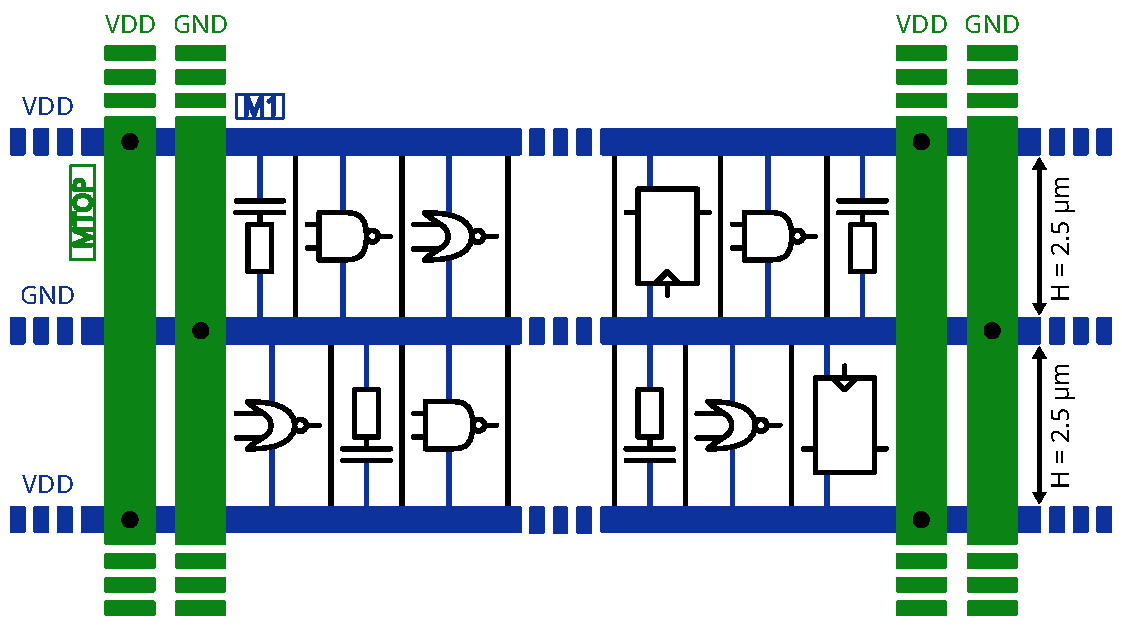
\includegraphics[width=0.49\textwidth]{./figures/psu_std_cell.pdf}
	\caption{A Standard-Cell Segment and its power delivery network.}
	\label{fig_alim_std}
\end{figure}

		The power distribution inside an IC is typically made with a grid-like structure, composed of metal wires stacked on top of each other on planes.
		The uppermost layer forms a ring surrounding the core.
		In each layer, the metal wires are equally spaced and have a dedicated width, which becomes thinner the deeper they are.
		The lowest layer brings the power directly to the transistors.
		
		Within these metal lines are located standard-cell segments (SCS), created by the power planning, as illustrated in Fig. \ref{fig_alim_std}.
		SCS are pre-characterized by foundries and classified according to their performance in timing and power consumption.
		Their height is fixed, while their width vary depending on their complexity, and are commonly made of logic gates, sequential, and decoupling elements.
	
		\subsubsection{Silicon substrate structure}
		Another important element of an IC is the substrate, and most importantly its type.
		We can mainly distinguish bulk and FD-SOI substrates.
		
		On the one hand, in bulk substrates, the transistor channel forms directly inside the P-substrate, and the depletion layer thickness is difficult to control.
		On the other hand, in FD-SOI substrates, a silicon oxide layer is created between the channel and the P-substrate, thus constraining the channel thickness.
		
		In this paper, we are focusing only on bulk substrates, and in this family, we can distinguish two substrate types: dual-well (DW) and triple-well (TW).
		The main difference between DW and TW substrates lies in how are lithographed NMOS transistors.
		In DW substrates, NMOS are located directly inside the P-doped substrate, and PMOS inside a N-doped well, called the N-well.
		However, in the case of a TW substrate, the PMOS are still inside the N-well, but the NMOS are located inside an additional P-doped well, made inside the N-well.
		
		These manufacturing differences are illustrated in Fig. \ref{fig_sub}, representing the cross-sectional view of an inverter made with a bulk technology.
		The PN and NP diodes formed between the substrate and the wells are represented, and the electrical resistances $R_C$ represent the access resistance of the substrate and the wells.
		% !TeX spellcheck = en_US
% !TeX root = ./0_article.tex

\begin{figure}[h]
	\centering
	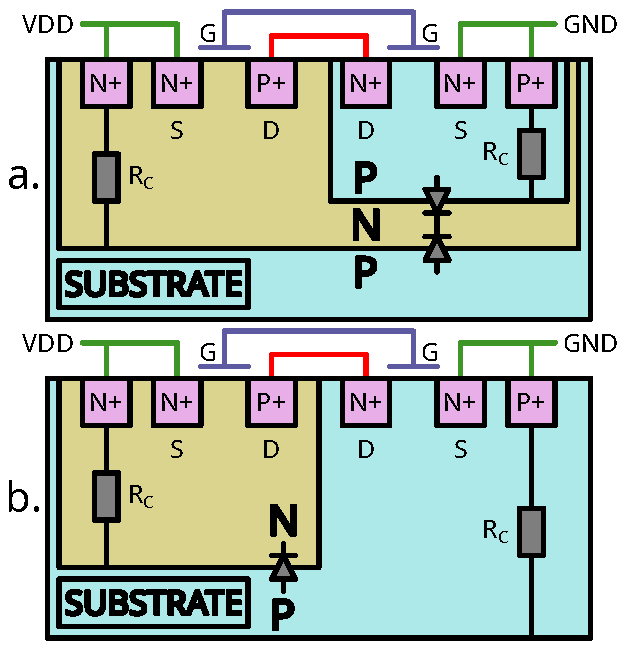
\includegraphics[width=0.35\textwidth]{./figures/substrate_2.pdf}
	\caption{Triple-well (a) and Dual-well (b) inverter cross-sectional view.}
	\label{fig_sub}
\end{figure}

		Dual-well substrates are found in moderately old ICs, while triple-well ones are common in more recent ICs, often coupled with dual-well substrate on the same die.
		The combination of both allows for \textcolor{orange}{cross-coupling noise reduction}, in addition to electrical insulation between transistors located on different domains (DW and TW).

		\subsubsection{Designing an elementary building-block for mass simulation}
		Thanks to the previously analyzed elements and models, we can now design elementary standard-cell blocks composed of the power delivery, the logic gates and the substrate, for each substrate type.
		As it has been said before, we are developing an hybrid simulation flow, therefore the designed elementary block is transistor-less.
		Eventually, our work is based on previous works on the subject \textcolor{cyan}{mathieuEMFI, FDTC2022, FDTC2023}.
		
		% !TeX spellcheck = en_US
% !TeX root = ./0_article.tex

\begin{figure*}[ht]
	\centering
	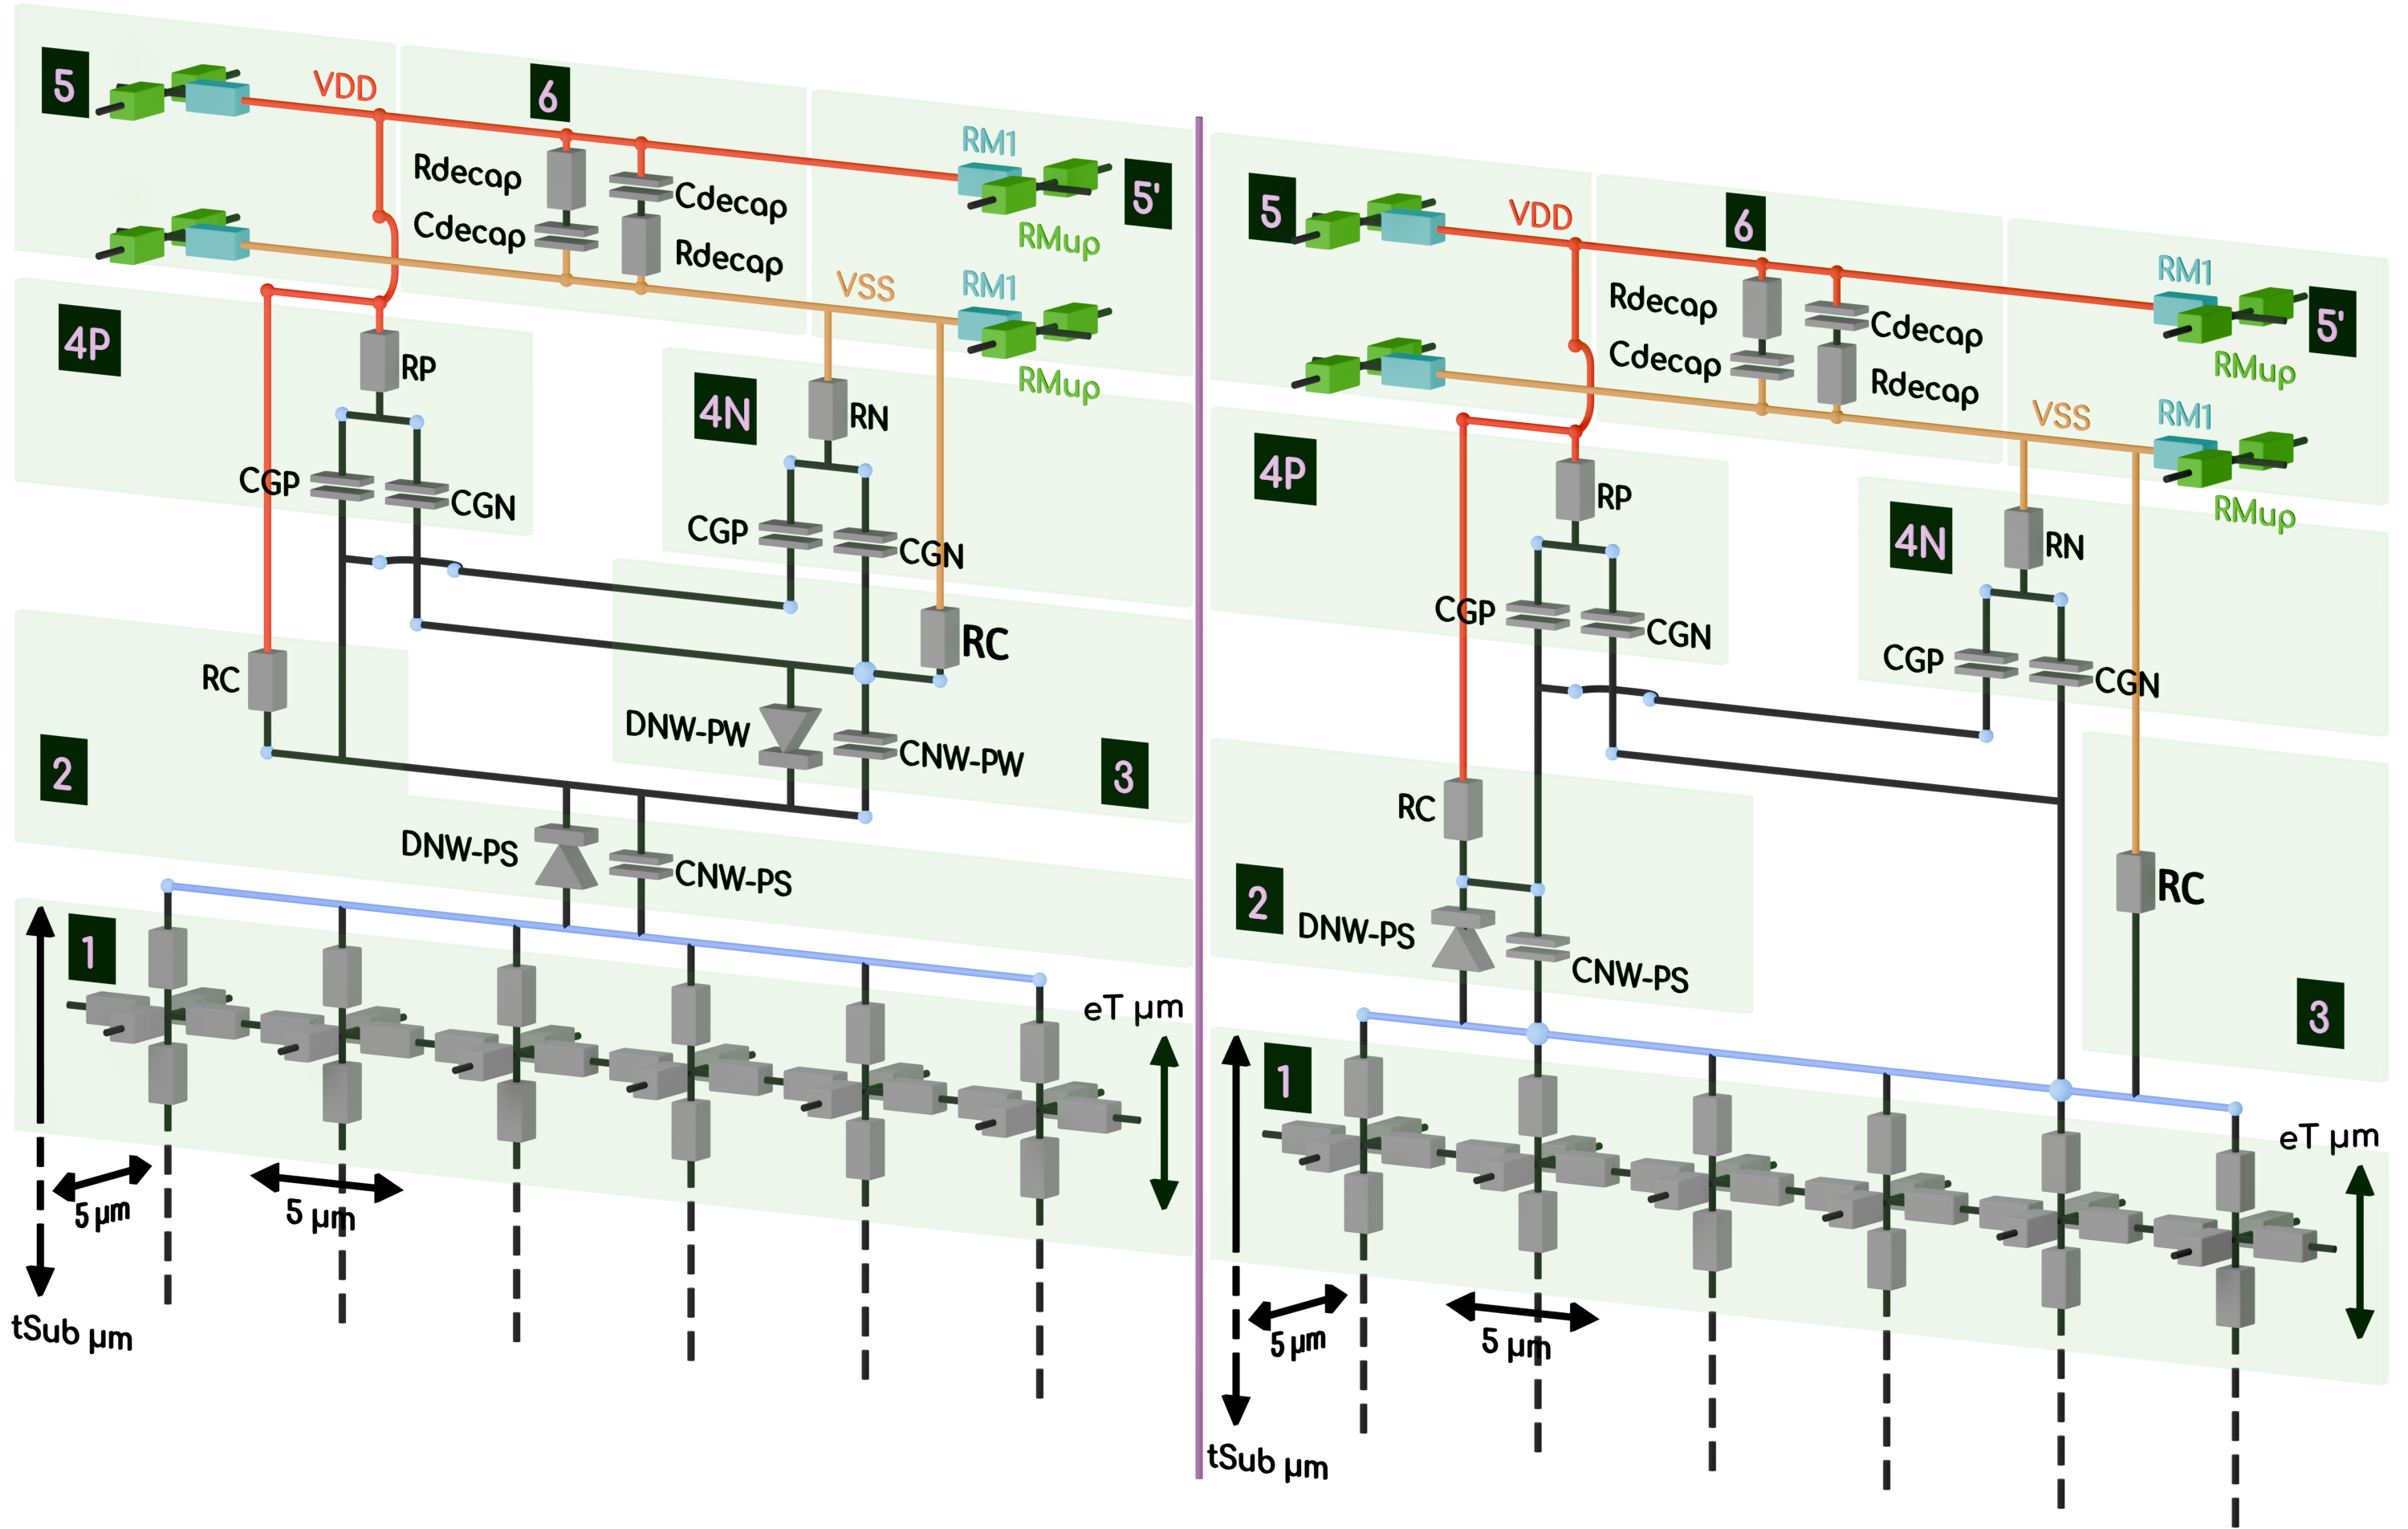
\includegraphics[width=0.95\textwidth]{./figures/dual+triple3.png}
	\caption{Triple well (left) and dual well (right) std cell \textcolor{red}{(PEUT ETRE FAIRE DES SOUS-FIGURES)}}
	\label{fig_triplewellstdcell}
\end{figure*}

		
		The model we propose is shown in Fig. \ref{fig_triplewellstdcell} both for a triple-well and a dual-well substrate.
		The models are extremely similar, but their difference is what is important.
		It represents an entire standard-cell segment, including a two levels power delivery network, average models of a hundred of logic gates, silicon junctions, and the silicon substrate.
		For better clarity, we divided the model into 6 sections, each representing a specific building block:
		\begin{itemize}
			\item \shadowbox{1} The substrate: modeled with 6 blocks of 6 resistors;
			\item \shadowbox{2} The P-N substrate-well silicon junction;
			\item \shadowbox{3} The N-P well-well silicon junction (TW), or the substrate access resistance (DW);
			\item \shadowbox{4N} \shadowbox{4P} The MOS average electrical model;
			\item \shadowbox{5} \shadowbox{5'} The power distribution metals;
			\item \shadowbox{6} The power supply decoupling.
		\end{itemize}
		The component values are calculated according to the target technology, in our case 90 nm, and are shown in Table \ref{tab_scs_numeric}

%\subsection{The hybrid simulation flow : building the models}
%The transistor-less model, also called standard-cell model, is developed thanks to the internal structure of integrated circuits, including:
%\begin{itemize}
%	\item Their power supply network;
%	\item Their standard-cells properties;
%	\item Their silicon substrate.
%\end{itemize}
%These three elements and their internal structure allow elaborating average models, able to represent their macro behavior.
%Fig. \ref{fig_alim_std} illustrates the base symbolic diagram used for our design.
%It represents a standard-cell segment, composed of logic gates and decoupling elements, with a fixed height of 5 µm and a variable width.
%For simplicity, two levels of metals for the power distribution are represented, the highest level MTOP in green and the first level M1 in blue.
%
%Then, because the previous analysis does not consider the substrate on which the transistors lie, it is required to extend the model.
%To that end, we represent in Fig. \ref{fig_sub} the cross-sectional view of a CMOS inverter in a triple-well and dual-well substrate.
%The parasitic silicon diodes formed between the substrate and the N-well, and between the N-well and the P-well are represented, in addition to the wells access electrical resistances $R_C$.
%
%Thanks to these preliminary analysis and former work on the subject \textcolor{cyan}{mathieuEMFI, fdtc20222023}, we set up an elementary transistor-less model, considering every presented aspect.
%This model, shown in Fig. \ref{fig_triplewellstdcell} for a triple-well substrate, represents a column portion of an IC, being 30 µm wide, 5 µm deep, and tSub µm thick.
%The schematic is divided into 6 sections:
%\begin{itemize}
%	\item \shadowbox{1} The substrate model, an array of distributed resistors;
%	\item \shadowbox{2} The P-N substrate-well silicon junction;
%	\item \shadowbox{3} The N-P well-well silicon junction;
%	\item \shadowbox{4N} \shadowbox{4P} The MOS average electrical model;
%	\item \shadowbox{5} \shadowbox{5'} The power distribution metals;
%	\item \shadowbox{6} The power supply decoupling.
%\end{itemize}
%The passive components modeling the transistors represent about 100 hundreds logic gates in the target technology.
%Therefore, the model allows evaluating simultaneously the average electrical behavior of 100 hundreds logic gates at a very low cost.
%
%% !TeX spellcheck = en_US
% !TeX root = ./0_article.tex
% LABEL AFTER CAPTION WESH GEOFFREY !!
\begin{figure}[h]
	\centering
	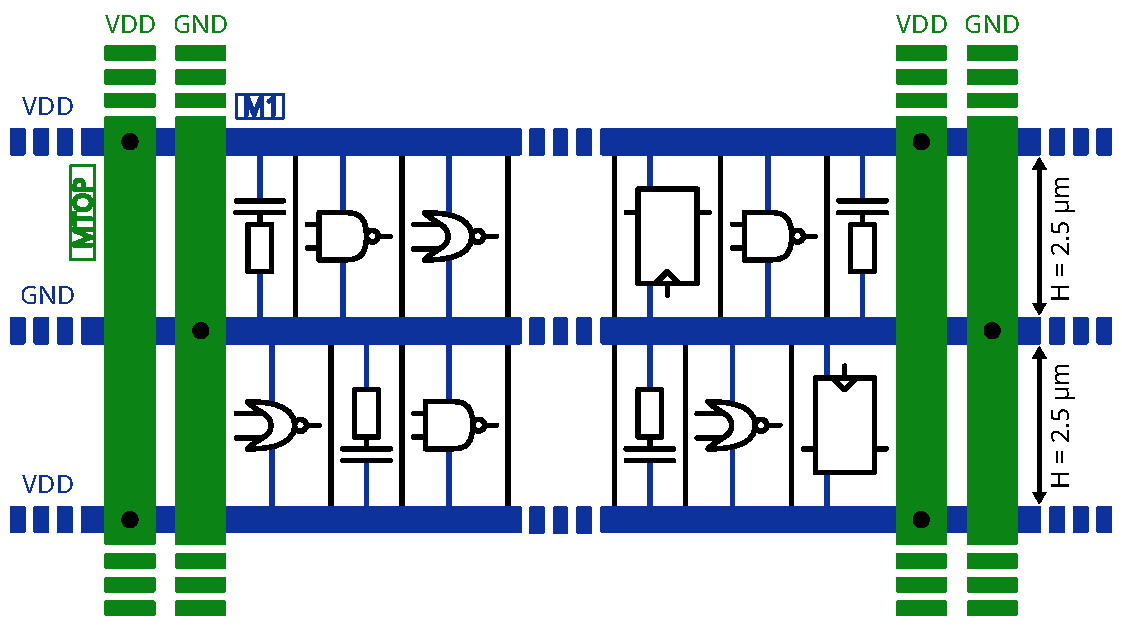
\includegraphics[width=0.49\textwidth]{./figures/psu_std_cell.pdf}
	\caption{A Standard-Cell Segment and its power delivery network.}
	\label{fig_alim_std}
\end{figure}

%
%% !TeX spellcheck = en_US
% !TeX root = ./0_article.tex

\begin{figure}[h]
	\centering
	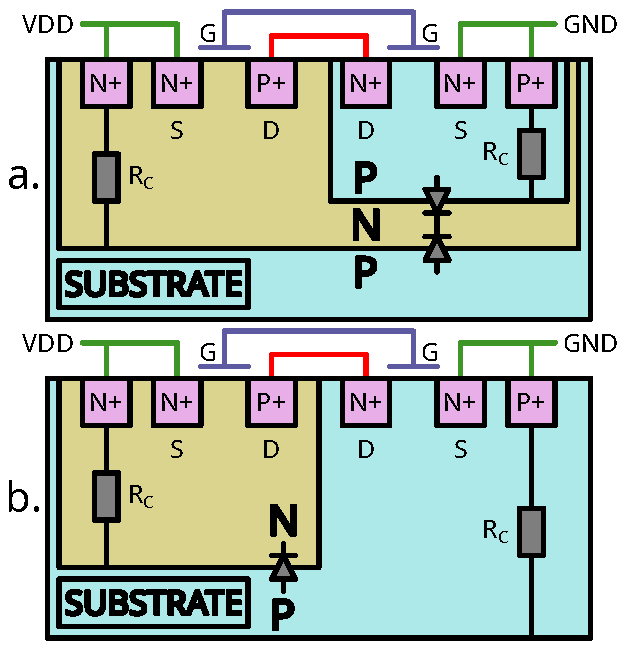
\includegraphics[width=0.35\textwidth]{./figures/substrate_2.pdf}
	\caption{Triple-well (a) and Dual-well (b) inverter cross-sectional view.}
	\label{fig_sub}
\end{figure}

%
%% !TeX spellcheck = en_US
% !TeX root = ./0_article.tex

\begin{figure*}[ht]
	\centering
	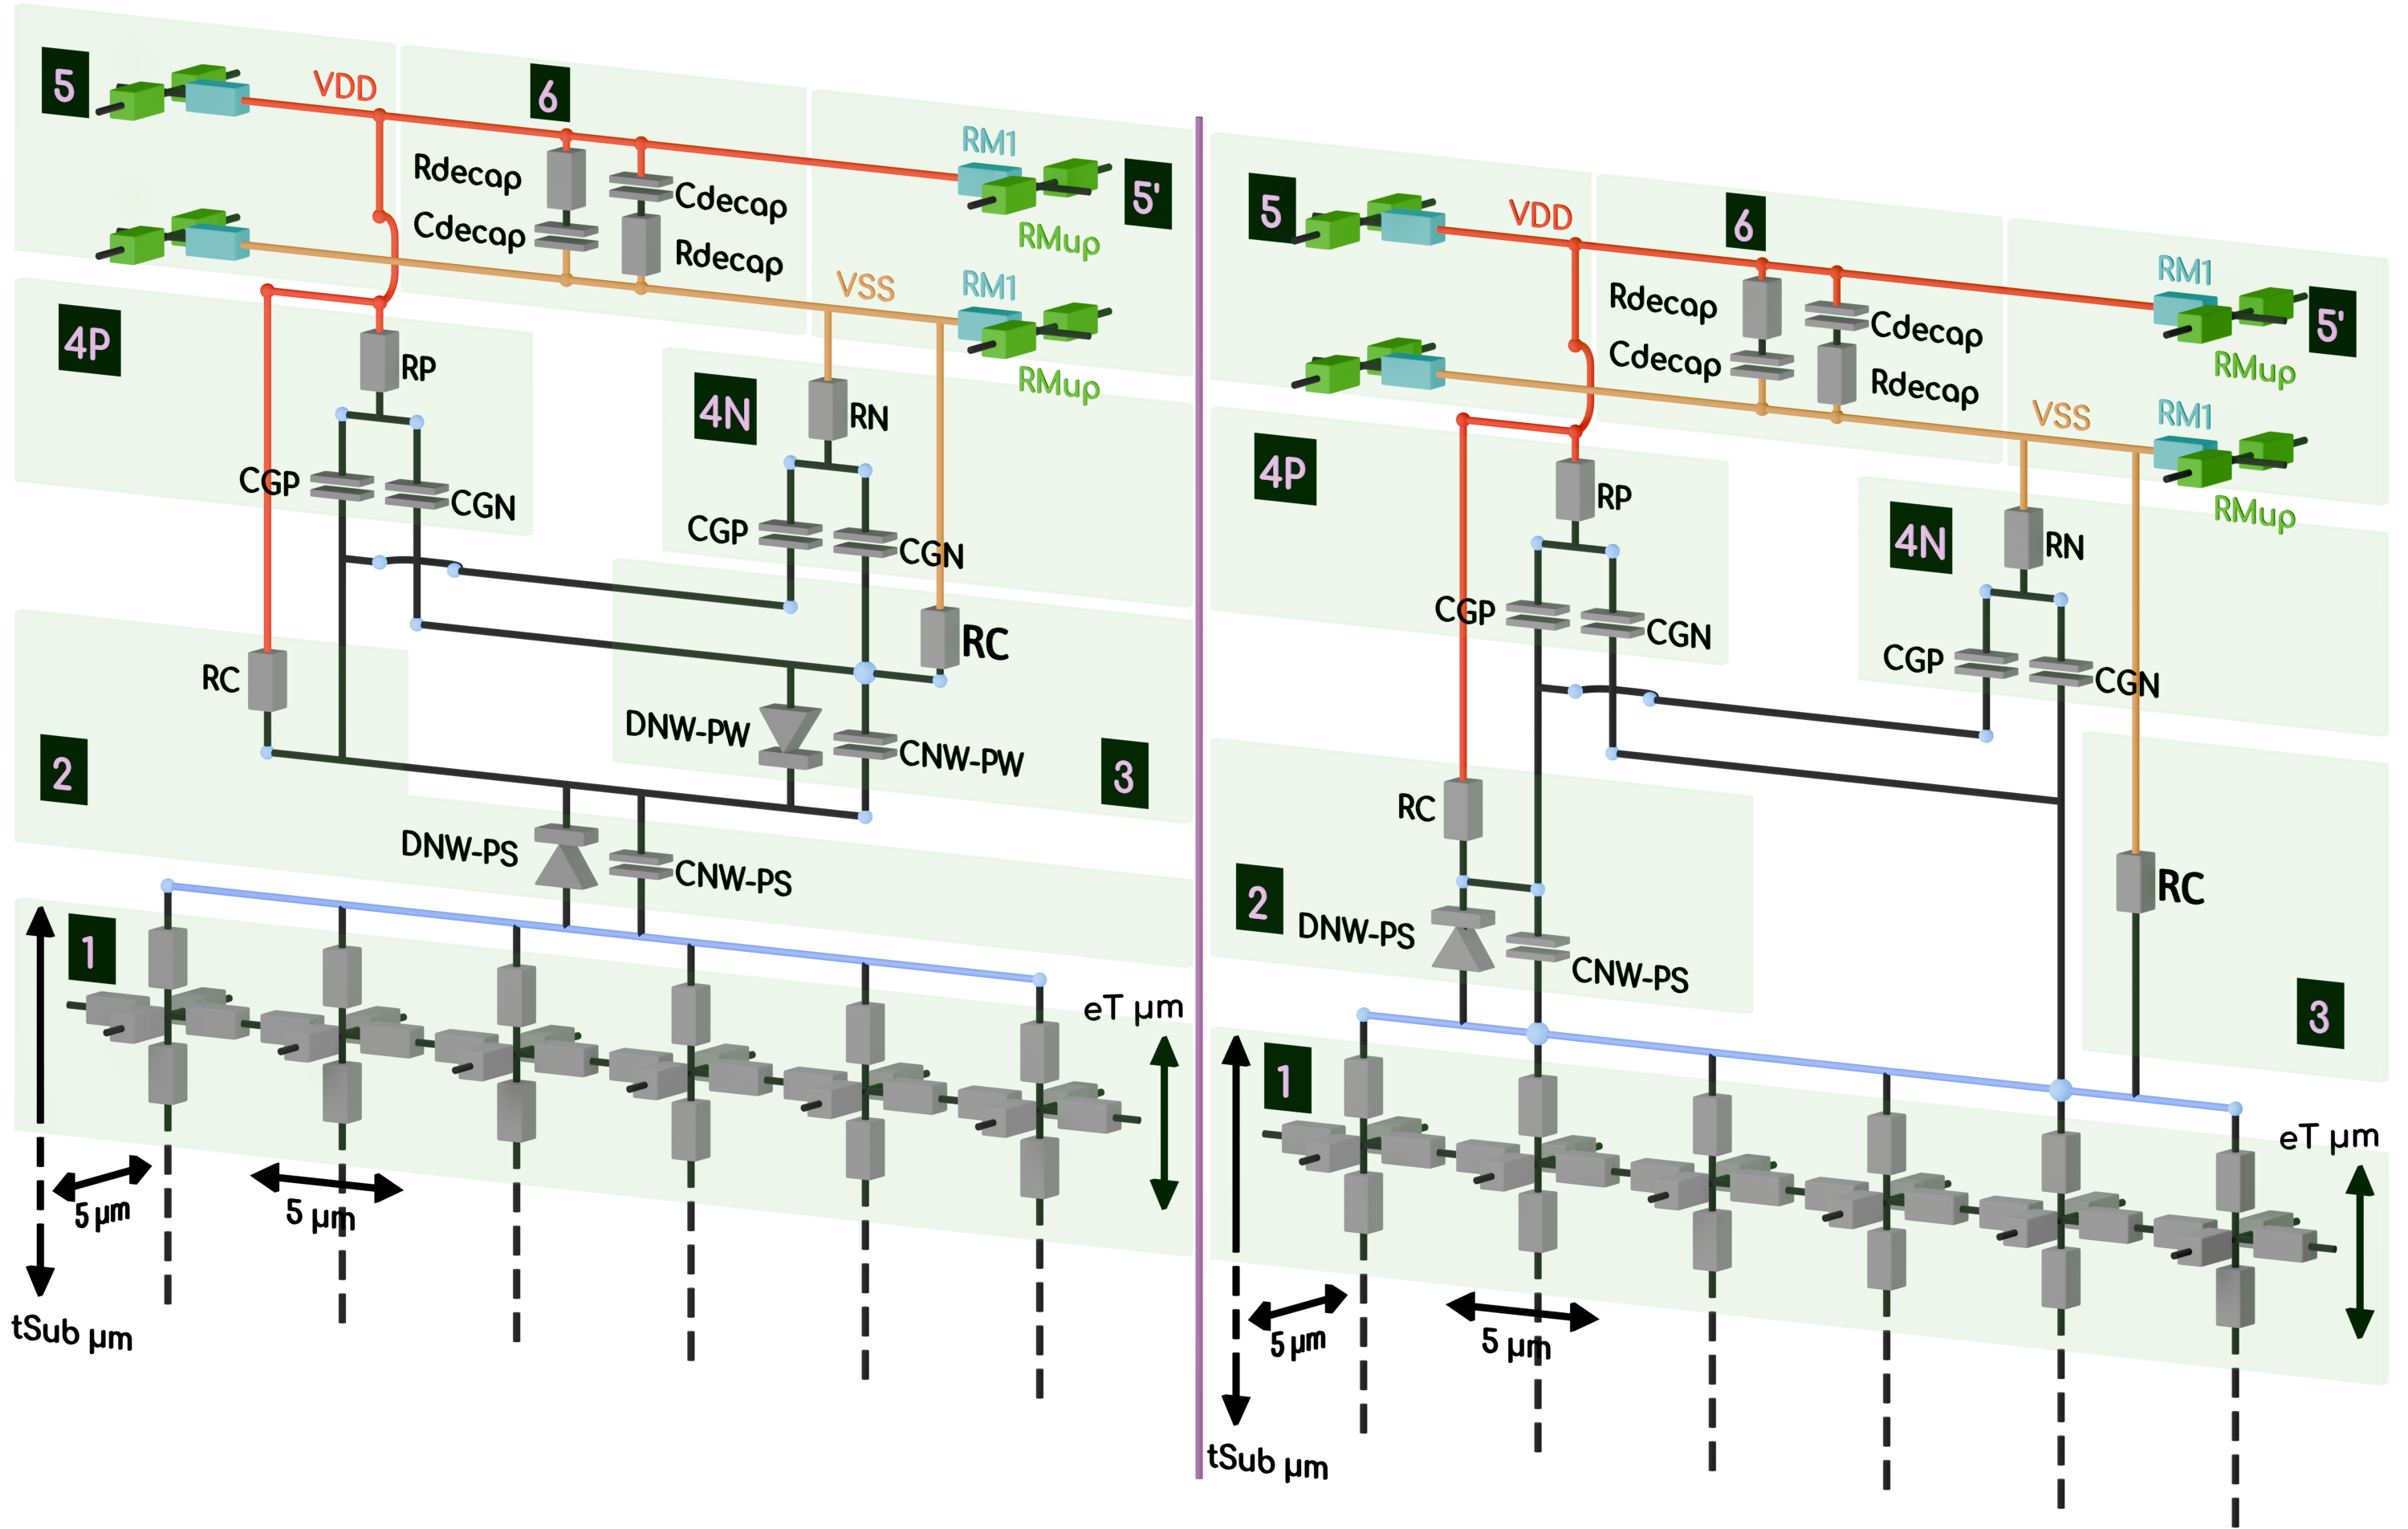
\includegraphics[width=0.95\textwidth]{./figures/dual+triple3.png}
	\caption{Triple well (left) and dual well (right) std cell \textcolor{red}{(PEUT ETRE FAIRE DES SOUS-FIGURES)}}
	\label{fig_triplewellstdcell}
\end{figure*}


%	% !TeX spellcheck = en_US
% !TeX root = ./0_article.tex

\section{Hybrid simulation results}

%	% !TeX root = ./0_article.tex

\section{Logic path under BBI}
For the purpose of analyzing the effects og BBI on actual logic, this section is dedicated in modeling and simulating an actual logic path
In this section, we are lingering on analyzing the effects of BBI on more complex logic paths.
The study is conducted for both a static logic path and a dynamic logic path.
The considered logic paths are constituted of inverters, buffers and a D-Flip-Flop (DFF).
The inverters model an arbitrary combinatorial logic path tackling the input of a DFF, used to sample the logic path output.
The DFF clock is buffered to achieve an isolation from the ideal voltage source.
Then, the DFF output is injected into a final 4-IVX chain, loaded with a 5 pF capacitor.
The resulting schematic is described in Fig. \ref{dffChain}.

\begin{figure}[h]
	\label{dffChain}
	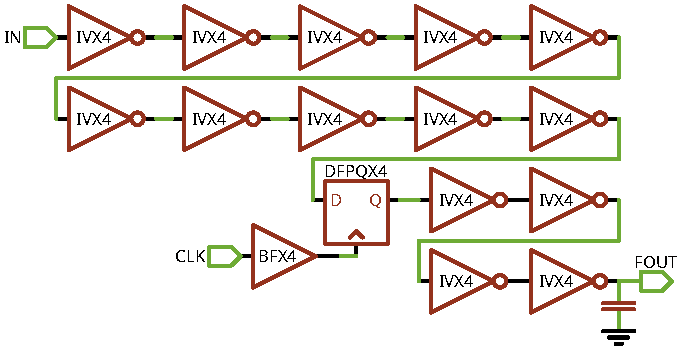
\includegraphics[width=0.5\textwidth]{./figures/dff_ivx_chain_2.pdf}
	\caption{DFFCHAIN}
\end{figure}

%	% !TeX root = ./0_article.tex

\section{Body biasing injection platforms overhaul}
\IEEEPARstart{T}{his} second section is dedicated in analyzing the various improvements we set up to enhance BBI reproducibility.
In the first place, we are going to analyze the various platforms proposed in the state-of-the art, then confront them to the proposed platform.
%	% !TeX spellcheck = en_US
% !TeX root = ./0_article.tex

\section{Conclusion}
	\IEEEPARstart{B}{ody} biasing injection has seen a re-emergence since 2020 \cite{bbiColin}, and various works have brought more and more knowledge throughout the years.
	BBI, contrary to EMFI or LFI, uses the silicon substrate of as the main physical medium to interact, transfer energy, and disturb integrated circuits.
	We introduced, through this work, the cumulative knowledge we gathered concerning BBI.
	This involves various aspects of the subjects.

	First, we studied better methods to improve BBI experiments repeatability and reliability through low-cost platform modifications.
	We supported these results with actual experiments such as Fault Analysis Mappings and a Differential Fault Attack.

	Then, we introduced large-scale IC modeling thanks to the use of transistor-less models allowing to reduce the computational power required to simulate BBI.

	Eventually, we extended this "transistor-less models" simulation flow to consider the logic functions of integrated circuits under BBI.
	This allowed us to understand the mechanisms at work during fault creation in integrated circuits under BBI, such as data-dependent bit set/reset faults, in addition to understanding the locality of BBI effects.

%	\begin{thebibliography}{1}
	\bibliographystyle{unsrt}
	\bibliography{references.bib}
%	\end{thebibliography}

\end{document}
